% TODO Check glossary entries (textbf stuff should probably be in glossary)!
\begin{fmffile}{feynman/LArTPC} % Open the feynman graph file
\fmfset{arrow_len}{2.5mm} % smaller arrows, default 4mm
\fmfset{zigzag_width}{1thick}
\fmfset{dash_len}{1.5mm}
\chapter{Working Principle of a Liquid Argon Time Projection Chamber} \label{sec:LArTPC}
The ultimate goal of every particle physics experiment is the measurement of an incident particle's energy, momentum vector, position in the detector, and finally its identity. In this chapter, I will show how a \gls{lartpc} achieves this goal. But first I give a brief overview of the history of the \gls{lartpc} and its operating principle. After this general review, I will present the working principles of a \gls{lartpc} in detail. As I view myself as a detector physicist and this chapter is close to my heart, I tried to properly research each topic in depths. During this process, I stumbled across several shortcomings and inconsistencies in our field which might be worthy of future studies.

In 1974 D. R. Nygren proposed a novel concept of a particle detector \cite{TPCProposal} to be built for the \gls{pep} collider experiment \cite{TPCExperiment} at \gls{slac}. The aim of this revolutionary detector setup was to provide a $4\pi$, truly 3-dimensional data signature with high spacial resolution, unambiguous spacial reconstruction and high data rate capability. In essence, Nygren's design was an ingenious application of a \gls{mwpc} \cite{TPCPredecessor} placed at the end of a large drift volume of methane gas as detector medium \cite{TPCDescription}, thus reducing the number of channels and simplifying reconstruction. He named his invention \gls{tpc}. Three years later C. Rubbia proposed the use of \gls{lar} as detector medium \cite{LArTPCProposal}, since it offers much higher density as methane gas. These \glspl{lartpc} can thus be used for low cross section experiments \eg neutrino detection. Moreover, \gls{lar}'s high density also provides a relatively high mass stopping power, and therefore excellent calorimeteric properties. As Argon is the third most abundant gas in our atmosphere and easily purified, its liquid form is available in large quantities for a low prise \cite{NobleGasDetectors}. These, and various other important properties of \gls{lar}, listed in table \ref{tab:LArProperties}, make it the material of choice for current and future neutrino experiments. Then, in 1982, P.J. Doe, H.-J. Mahler, and H.H. Chen built and operated the first \gls{lartpc}, measuring tracks in two dimensions (only one wire-plane) \cite{LArTPCFirst}. Three years later Rubbia and the ICARUS collaboration proposed the first large scale \glspl{lartpc} to be situated in the Gran Sasso Laboratory deep underground \cite{ICARUSProposal}. This marked the beginning of various important developments in material testing and cryogenics by said collaboration, resulting in the modular ICARUS T600 detector commissioned in 2004 \cite{ICARUST600}. The ICARUS T600 consisted of two T300 modules with a total active detector mass of \SI{476}{\tonne}. All large scale designs following ICARUS were heavily influence by this detector design, and so was MicroBooNE, although not matching the uncompromising build quality of ICARUS. 
% TODO Add more history: Argontube? ArDM?

Before a \gls{lartpc} can be operated, the detector medium, \gls{lar}, needs to be contained and kept at constant temperature. Therefore, thermally insulated cryogenic steel vessels of various designs are used. In these vessels the \gls{tpc} usually rests on electrically insulating holding structures. Every \gls{tpc} has a so-called \textbf{active volume} in its core, filled with the detector medium, like \gls{lar}, where the particle interactions take place. In said active volume a constant and uniform electric field is applied between an anode and a cathode, wherefore a field cage surrounding the active volume is employed. The field cage is usually charged by a \gls{dc} \gls{hv}, fed through the cryogenic vessel and stepped down by resistors between every field cage stage. A \gls{tpc}'s anode also acts as its readout system. So far, all large scale detectors employ multi-wire planes able to measure the charge of particle's ionisation traces. Finally, \glspl{lartpc} feature a light readout system, usually consisting of \glspl{pmt}. A schematic view of an above described \gls{lartpc} is shown in figure \ref{fig:TPCSchematics}.
\begin{figure}[htbp]
    \centering
    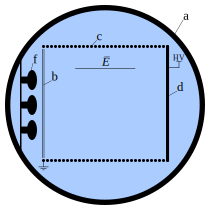
\includegraphics[width=0.9\textwidth]{images/Detector/TPCSchematics.pdf}
    \caption[Schematic view of a LArTPC]{Schematic side view of a \gls{lartpc}. In this picture, \textbf{a} is the vessel containing the \gls{lar} (light blue) and the \gls{tpc}. At letter \textbf{b} the readout planes are positioned, in this case depicted as three wire planes in various orientations. The readout planes also act as the anode of the \gls{tpc}. Labelled by \textbf{c}, one finds the field cage comprised of single steel tubes connected by a voltage divider, \ie the voltage decreases with every tube towards the anode. The cathode is labelled by \textbf{d}, so \textbf{b} through \textbf{d} show all the components of a \gls{tpc} and enclose the active volume. Applying a negative \gls{hv} to the cathode introduces an uniform electric field $\vec{E}$ pointing from the anode to the cathode. Finally, \textbf{f} shows the light readout system, in this case an array of \glspl{pmt}.}
    \label{fig:TPCSchematics}
\end{figure}

As a charged particle traverses the active volume it ionises the detection medium (\gls{lar}) along its trajectory and also creates excited states, see figure \ref{fig:TPCFunction1}. Thereupon a fraction of the resulting electron-ion pairs recombine and thus produce more excited states. Most of these then decay under the emission of scintillation light, while some come in contact with impurities and decay emitting heat. The whole recombination and scintillation process occurs within a time scale of nanoseconds. A light readout system, historically consisting of multiple \glspl{pmt}, is then used to detect said light emission in order to determine the time $t_0$ of the incident particle crossing the active volume. These recombination and scintillation mechanisms are all shown in figure \ref{fig:TPCFunction2}. Yet, the electric field $\vec{E}$ prevents a full recombination and lets the electrons drift towards the anode with a constant velocity $v_\text{d}$ and the ions, although much slower, towards the cathode. During the drift, some of the electrons get captured by impurities, as depicted figure \ref{fig:TPCFunction3}. When the electrons reach the anode, the readout wire planes detect the drift charges, as visualised in figure \ref{fig:TPCFunction4}. These wire plane signals are then used to measure the \gls{2d} positioning $(y,z)$, timing $t$, and intensity of the incoming drift electrons. The electron drift time, $t-t_0$, is of the order milliseconds for large scale detectors. Knowing the drift velocity $v_\text{d}$, $t-t_0$ can be used to calculate the missing coordinate $x = v_\text{d}(t-t_0)$ and thus, in combination with the \gls{2d} positioning, one obtains a \gls{3d} interaction picture $(x,y,z)$ of the incident particles. Furthermore, the measured charge intensity facilitates particle identification and calorimetry. In the following subsections the abovementioned working principle of a \gls{lartpc} will be discussed in depth, based on the works of E. Aprile, A. E. Bolotnikov, A. I. Bolozdnya, and T. Doke \cite{NobleGasDetectors} as well as V. Chepel and H. Ara\'ujo \cite{NobleGasDetectorsBetter}.
\begin{figure}[htbp]
    \centering
    \subfloat[Ionisation and Excitation][Ionisation and excitation]
    {
        \includegraphics[width=0.48\textwidth]{images/Detector/TPCFunction1.pdf}
        \label{fig:TPCFunction1}
    } %\qquad
    \subfloat[Recombination and Scintillation][Recombination and scintillation]
    {
        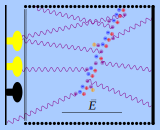
\includegraphics[width=0.48\textwidth]{images/Detector/TPCFunction2.pdf}
        \label{fig:TPCFunction2}
    } \\
    \subfloat[Electron- and Ion Drift][Electron- and ion drift]
    {
        \includegraphics[width=0.48\textwidth]{images/Detector/TPCFunction3.pdf}
        \label{fig:TPCFunction3}
    } %\qquad
    \subfloat[Charge Signal Readout][Charge signal readout]
    {
        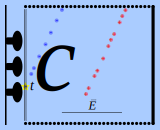
\includegraphics[width=0.48\textwidth]{images/Detector/TPCFunction4.pdf}
        \label{fig:TPCFunction4}
    }
    \caption[Working Principle of a Liquid Argon TPC]{In the above figures the working principle of a \gls{lartpc} is illustrated. In \subref{fig:TPCFunction1} the ionisation and excitation process is depicted, as a charged particle enters the active volume, with its trajectory illustrated in green. Along said trajectory electrons (blue spots), argon ions (red spots), and excited states of argon (purple spots) are created by the incident particle's energy deposition. Image \subref{fig:TPCFunction2} shows the recombination- and scintillation light creation processes. Here, some of the electrons and ions recombine to form more excited states, but the electric field $\vec{E}$ prevents all of them from recombining. Almost instantly a majority of the excited states are involved in the production of scintillation photons (purple wavy lines), while some are quenched by impurities (orange spots) or argon ions. If the photons hit the \glspl{pmt} of the light readout system, these then generate a time signal $t_0$ (indicated as yellow \glspl{pmt}). In \subref{fig:TPCFunction3} the electron and ion drift are depicted. While the electron drift, due to $\vec{E}$, with a constant velocity $v_\text{d}$ towards the anode, they sometimes get captured by impurities with a high \gls{electronegativity} (orange spots) and are thus becoming useless for the charge signal measurement. The argon ions drift much slower towards the cathode. Finally, depicted in \subref{fig:TPCFunction4} is the charge signal creation at the readout plane. When the electrons reach the readout plane at the anode end of the \gls{tpc}, they generate a signal (yellow star) in \gls{2d} space $(y,z)$, arrival time $t$, and amount of charge. The arrival time can be used in combination with $t_0$ and $v_\text{d}$ to reconstruct the third spacial component $x = v_\text{d}(t-t0)$. The resulting signal is a \gls{3d} picture, $(x,y,z)$, of the incident particle track and its energy deposition.}
    \label{fig:TPCFunction}
\end{figure}

\section{Liquid Argon Properties}
There are several advantageous properties of \gls{lar} which makes it preferable for the use as a \gls{tpc} medium. Most notably, noble gases like argon are inert substances featuring a fully occupied valence shell. Therefore they neither bond with, nor attract \glspl{quasifreeelectron}. Heavy noble liquids and solids (argon, krypton, and xenon) feature a high polarisability, thus allowing for \glspl{quasifreeelectron} to drift with high velocities. This property allows for long drift distances (tens of meters). Another advantages property of noble liquids in general is their translucence to their own scintillation light. In all the aforementioned properties xenon excels all the other noble liquids, but argon is the third most abundant gas in the atmosphere and thus the noble gas with the lowest cost associated to it. This makes \gls{lar} the only affordable option for the use in multi-kiloton detectors.

However, there are also several challenges associated with the use of \gls{lar}. A major concern is the relatively low \gls{bp} of $T_{\text{b}}=\SI{87.303(2)}{\kelvin}$ at standard pressure. This requires the utilisation of complicated cryogenic systems in order to establish a controlled detector environment. Furthermore, with a \gls{mp} of $T_{\text{m}} = \SI{83.8(3)}{\kelvin}$ the temperature range of the liquid state amounts only to \SI{3.5(3)}{\kelvin}, which further complicates the cryogenic requirements. The thermodynamic properties argon are listed in table \ref{tab:LArProperties} and shown in the phase diagram in figure \ref{fig:PhaseDiagram}.
\begin{figure}[htbp]
    \centering
    \includegraphics[width=0.9\textwidth]{images/Detector/PhaseDiagramArgon.pdf}
    \caption[Phase Diagram of Argon]{Phase diagram of argon in the temperature-pressure space in the ranges of \SIrange{60}{180}{\kelvin} and \SIrange{1e-2}{1e4}{\bar}. The lines of phase changes are drawn in colour and the standard pressure as a dashed line at \SI{1}{\bar}. Where the latter crosses the phase change lines the \acrfull{bp} and \acrfull{mp} are highlighted. The \acrfull{tp} and \acrfull{cp} are shown as well. Formulas and values were sourced from \cite{ArgonProperties2,ArgonProperties3}.}
    \label{fig:PhaseDiagram}
\end{figure}
Other difficulties are not posed by the \gls{lar} itself, but by three impurity types: 
\begin{itemize}
    \item Radioactive isotopes, which mimic low energy light and charge signals. These consist mostly of radon introduced through outgassing of contaminated solids like glass. Another source of radio activity is posed by radioactive argon isotopes, most prominently \ce{^39Ar} with a $T_{1/2}=\SI{269(3)}{\year}$ \cite{IsotopeData}. 
    \item Scintillation light quenching impurities, which reduce the light intensity measured by the light readout system. During standard operations the main contributor for this is nitrogen \ce{N2}.
    \item Charge binding impurities which reduce the charge collected by the readout. These are mostly molecules composed of atoms with high \gls{electronegativity} like \ce{O2} or \ce{H2O}.
\end{itemize}
However, all these operational difficulties can be controlled by filtering techniques, smart choice of materials, underground argon, and cleanliness during installation. Thus \gls{lar} serves as an excellent detector medium in \glspl{tpc}. The \gls{lar} properties most essential for \gls{lartpc} operations are listed in table \ref{tab:LArProperties}.

In regards of safety, the low \gls{bp} of argon may lead to fast pressurisation of any storage vessel. This could lead to catastrophic explosions if left unmitigated. Thus safety release valves and rupture discs, which vent the gas in an emergency, are paramount for safe \gls{lartpc} operations. In gas form, argon's high density lets it displace air and creating an oxygen deficiency hazard in underground facilities and other confined spaces. This is mitigated by workers safety training, wearing of oxygen monitors, as well as ventilation systems providing a safe path to emergency exits. It is therefore possible to safely operate even large scale \glspl{lartpc}.

\begin{table}[hbtp]
    \centering
    \caption[Properties of Liquid Argon]{Properties of liquid argon. For the mean excitation energy only the value of the gas phase is available (for liquid \ce{H2} it is increased by $\sim\SI{14}{\percent}$ compared to gas \cite{StoppingPowerNumbers}). The acronym \acrshort{mip} stands for \acrlong{mip} which will be explained later in this chapter.}
    \begin{tabu} to 0.7\textwidth{lcrlc} \toprule
        \rowfont[c]{\bf} Variable & Symbol & Value & Unit & Source\\ \midrule
        Atomic number & $Z$ & 18 & & \cite{ArgonProperties1}\\
        Molecular weight & $A$ & \num[separate-uncertainty = false]{39.948(1)} & \si{\gram\per\mol} & \cite{ArgonProperties1} \\
        \Acrfull{bp} at \SI{1}{\bar}& $T_{\text{b}}$ & \num[separate-uncertainty = false]{87.303(2)} & \si{\kelvin} & \cite{ArgonProperties2} \\
        \Acrfull{mp} at \SI{1}{\bar}& $T_{\text{m}}$ & \num[separate-uncertainty = false]{83.8(3)} & \si{\kelvin} & \cite{ArgonProperties3} \\ 
        Density at \SI{1}{\bar} \gls{bp} & $\rho$ & \num{1.39646} & \si{\gram\per\centi\metre\cubed} & \cite{ArgonProperties2} \\ 
        Viscosity at \SI{1}{\bar} \gls{bp} & $\eta$ & \num[separate-uncertainty = false]{273.2(55)} & \si{\micro\pascal\second} & \cite{NistChemistryWebBook} \\ 
        Sound velocity at \SI{1}{\bar} \gls{bp} & $c_\text{s}$ & \num[separate-uncertainty = false]{842.9(84)} & \si{\metre\per\second} & \cite{NistChemistryWebBook} \\ \midrule
        \multirow{2}{*}{\Acrfull{tp}} & $T_{\text{t}}$ & \num{83.8058} & \si{\kelvin} & \multirow{2}{*}{\cite{ArgonProperties2}} \\
                                      & $p_{\text{t}}$ & \num[separate-uncertainty = false]{0.68891(2)} & \si{\kilo\pascal} & \\ \midrule
        \multirow{2}{*}{\Acrfull{cp}} & $T_{\text{c}}$ & \num[separate-uncertainty = false]{150.687(15)} & \si{\kelvin} & \multirow{2}{*}{\cite{ArgonProperties2}}  \\
                                      & $p_{\text{c}}$ & \num[separate-uncertainty = false]{48.63(3)} & \si{\bar} &  \\ \midrule
        Ionisation energy (gas) & $I_\text{GAr}$ & \num[separate-uncertainty = false]{15.7596099(7)} & \si{\electronvolt} & \cite{ArgonIonisationEnergy}\\
        Ionisation energy (liquid) & $I_{\text{LAr}}$ & \num{13.4} & \si{\electronvolt} & \cite{NobleGasDetectors} \\
        W-value of ionisation & $W_\text{i}$ & \num[separate-uncertainty = false]{23.6(3)} & \si{\electronvolt} & \cite{LArW-Value,LArW-ValueErratum} \\
        W-value of scintillation (max) & $W_\text{ph}(\text{max})$ & \num[separate-uncertainty = false]{19.5(10)} & \si{\electronvolt} & \cite{LArWScint-Value1,LArWScint-Value2} \\
        W-value of scint. (\acrshort{mip}) & $W_\text{ph}(\text{MIP})$ & \num[separate-uncertainty = false]{25.1(25)} & \si{\electronvolt} & \cite{LArWScint-Value1,LArWScint-Value2} \\
        Scintillation wave length & $\lambda_\text{sc}$ & \num[separate-uncertainty = false]{128(10)} & \si{\nano\metre} & \cite{LArScintillationSpectrum1,LArScintillationSpectrum2} \\
        Mean excitation Energy (gas) & $I_{\text{ex}}$ & \num[separate-uncertainty = false]{188(10)} & \si{\electronvolt} & \cite{StoppingPowerNumbers} \\
        Critical Energy of $e^{-}$ & $E_\text{c}$ & \num{32.84} & \si{\mega\electronvolt} & \cite{PDGMaterialProperties} \\
        Radiation length & $X_0$ & \num{19.55} & \si{\gram\per\centi\metre\squared} & \cite{PDGMaterialProperties} \\ %TODO check if more reliable source?
        Dielectric constant & $\epsilon_\text{r}$  & \num[separate-uncertainty = false]{1.504(1)} & & \cite{LArDielectricConstant} \\
        Refractive index at \SI{546.1}{\nano\metre} & $n$  & \num[separate-uncertainty = false]{1.2278(12)} & & \cite{LArRefractiveIndex} \\
        Moli\`{e}re radius & $R_\text{m}$ & \num{9.043} & \si{\centi\metre} & \cite{PDGMaterialProperties} \\
        \acrshort{mip} linear stopping power & $\left\langle -\frac{dE}{dx} \right\rangle_\text{MIP}$ & \num{2.105} & \si{\mega\electronvolt\per\centi\metre} & \cite{PDGMaterialProperties} \\
        \bottomrule
    \end{tabu}
    \label{tab:LArProperties}
\end{table}
% TODO sort table!!!!!

% Particles in Argon
\section{Excitation and Ionisation of Liquid Argon} \label{sec:ParticleInteractions}
Only charged particles can be directly observed in a \gls{lartpc}, as they interact with the detector medium through Coulomb forces. In essence, there are three immediate effects a charged particle, here denoted as \ce{X^{$\pm$}}, has on an argon atom \ce{Ar}. The first and lowest energy process, is the excitation of the atom, denoted by \ch{Ar^*}. The second interaction mode, requiring more energy than excitation, is producing an electron-ion pair, \ie ionisation. The resulting charged ion is represented by the symbol \ce{Ar^+}. Finally there is the spallation of the atom by direct interaction with its core. This produces a multitude, \ia of charged particles, which are again subject to the former two interactions. However, spallation requires many orders of magnitudes more energy (at least several \SI{100}{\mega\electronvolt}) than ionisation (around \SI{10}{\electronvolt}) or excitation (several \si{\electronvolt}). In this work, I will present the latter two interactions, and omit an in depth discussion of spallation. 

The ionisation, as mentioned before, is induced by a charged particle, \ce{X^{$\pm$}}, transferring momentum to an electron, in the shell of an argon atom, \ce{Ar}, by the means of the \gls{em} force. Consequently, the electron overcomes the Coulomb-potential of the atom which results in a \gls{quasifreeelectron} $e^-$ and a positively charged argon ion \ce{Ar^+}. We can thus express said process by
\begin{equation} \label{eq:IonisationProcess}
    \ce{Ar + $X^{\pm}$ -> Ar^+ + $e^-$ + $X^{\prime\pm}$}.
\end{equation}
In this case, \ce{X^{$\prime\pm$}} stands for the ionising particle \ce{X^{$\pm$}} after the energy loss. The excitation process is very similar with the difference that the transferred energy is too low to overcome the Coulomb-potential and thus placing the electron only on a higher energy eigenstate, \ie an excited state. The production of an excited argon atom \ch{Ar^*} can be described as
\begin{equation} \label{eq:ExcitationProcess}
    \ce{Ar + $X^{\pm}$ -> \ch{Ar^*} + $X^{\prime\pm}$}.
\end{equation}
In addition there are also occurrences of multiply ionised states \ce{Ar^{$n$+}}, excited ionised states \ch{Ar^{+*}}, as well as combinations of the two:
\begin{align} \label{eq:SecondaryIonProcess}
    \ce{Ar + $X^{\pm}$ &-> Ar^{$n$+} + $n e^-$ + $X^{\prime\pm}$}, \nonumber \\
    \ce{Ar + $X^{\pm}$ &-> \ch{Ar^{+*}} + $e^-$ + $X^{\prime\pm}$}, \\
    \ce{Ar + $X^{\pm}$ &-> \ch{Ar^{$n$+*}} + $n e^-$ + $X^{\prime\pm}$}. \nonumber
\end{align}
In a Feynman diagram the ionisation and excitation processes look the same, for both are momentum transfers from $X^{\pm}$ to the electron $e^-$ in the atomic shell. The momentum is transferred by a photon as illustrated in figure \ref{fig:IonisationAndExcitation}.
\begin{figure}[htbp]
    \centering
    \fmfframe(10,10)(0,10){
        \begin{fmfgraph*}(120,80)
            \fmfleft{i1,i2}
            \fmfright{o1,o2}
            \fmf{fermion}{i1,v1,o1}
            \fmf{fermion}{i2,v2,o2}
            \fmf{photon,label=$\gamma$,label.side=left,label.dist=0.1cm}{v1,v2}
            \marrow{photm}{right}{rt}{$p$}{v2,v1}
            \fmfv{label=$e^-$,label.angle=180,label.dist=0.1cm}{i1}
            \fmfv{label=$X^\pm$,label.angle=180,label.dist=0.1cm}{i2}
            \fmfv{label=$e^-$,label.angle=0,label.dist=0.1cm}{o1}
            \fmfv{label=$X^{\prime\pm}$,label.angle=0,label.dist=0.1cm}{o2}
            \fmfv{decor.shape=circle,decor.filled=full,decor.size=1thick}{v1}
            \fmfv{decor.shape=circle,decor.filled=full,decor.size=1thick}{v2}
        \end{fmfgraph*}
    }
    \caption[Feynman Diagrams of Ionisation and Excitation]{This figure depicts the Feynman diagrams of the ionisation and excitation process. In processes the momentum $p$ is transferred from a charged particle $X^{\pm}$ to a shell electron $e^-$ by a photon $\gamma$.}
    \label{fig:IonisationAndExcitation}
\end{figure}

The rate of ionisation or excitation is not only depending on the momentum transferred by the charged particle, but also by the ionisation potential and resonant energy levels of \gls{lar} as well as their structure. In a condensed, non-polarised, dense fluid, like \gls{lar}, one observes a reduction in ionisation energy compared to their gas state, \ie  $I_\text{liquid} < I_\text{gas}$. This is attributed to three effects:
\begin{enumerate}
    \item The conduction band of the quasi-free electrons widens, thus, effectively reducing the ionisation threshold by the band's width $V_0$.
    \item The higher atomic density of a liquid leads to an increase of the dielectric constant $\epsilon_\text{r}$, hence, raising the polarisability of the single atoms. This elevates the ground state energy of the valence electrons by the polarisation energy $P_+$.
    \item The valence electron energy levels develop into valence bands, increasing the ground state energy by the band's width $E_\text{val}$.
\end{enumerate}
With this information we can now form a rather simple equation for calculating the ionisation energy of a non-polarised liquid \cite{LArIonisationEnergy1},
\begin{equation} \label{eq:LiquidIonisationEnergy}
    I_\text{liquid} = I_\text{gas} + V_0 + P_+ + E_\text{val}.
\end{equation}
Here the signs are positive by convention, and thus, $V_0$, $P_+$, and $E_\text{val}$ all take negative values. Above effects and equation are schematically depicted in figure \ref{fig:LArIonisationPotential}.
\begin{figure}[htbp]
    \centering
    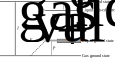
\includegraphics[width=0.9\textwidth]{images/Detector/LArIonisationPotential.pdf}     
    \caption[Changes in the Ionisation Energy Induced by Condensation]{This picture shows a schematic representation of the changes to the ionisation energy induced by condensation. In non-polarised liquids the ionisation energy is reduced compared to the gas state, $I_\text{liquid} < I_\text{gas}$. This is explained by the reduction of the ground state energy of quasi-free electrons $V_0$, the increase of the ground state energy level by the polarisation energy $P_+$, and the development of valence band with a width of $E_\text{val}$. The band gaps in above depiction are not to scale. This graph is inspired by \cite{LArIonisationEnergy2}.}
    \label{fig:LArIonisationPotential}
\end{figure}
By far the largest contributing factor to the ionisation energy shift is the polarisation energy $P_+$ typically ranging between \SIrange{1}{2}{\electronvolt} \cite{LArIonisationEnergy2}. $P_+$ can be derived employing the Born equation \cite{BornEquation} which is just the difference between the potential energies of a singly charged sphere with radius $r_+$ in vacuum $W(\epsilon_0)$ and in a medium $W(\epsilon_0\epsilon_\text{r})$:
\begin{equation}
    P_+ = \frac{1}{2} \left( W(\epsilon_0\epsilon_\text{r}) - W(\epsilon_0) \right) = - \frac{e^2}{8 \pi \epsilon_0 r_+} \left( 1 - \frac{1}{\epsilon_\text{r}} \right).
\end{equation}
Here $\epsilon_\text{r}$ denotes the dielectric constant of the medium, in our case \gls{lar}, $\epsilon_0$ the vacuum permittivity, and $e$ the electron charge. Besides these often used constants there is also $r_+$ which stand for the radius of a singly ionised atom of the medium. Above equation indicates that the $P_+$ correction is just the classical approximation of the behaviour of the outermost electron in the ion's potential while changing the dielectric constant. Note that, according to equation \ref{eq:LiquidIonisationEnergy}, this classical correction is then applied to shift quantum mechanical energy eigenstates; quite an oddity in physics. As for $V_0$ and $E_\text{val}$, these both have to be measured and their values are usually one order of magnitude smaller than $P_+$. In addition to the shift in ionisation potentials, when condensing a gas into a liquid, the excited states are also affected. Their energy levels are shifted by the same energy difference $\Delta I = I_\text{liquid} - I_\text{gas}$. Furthermore, the levels also broaden and form bands, just like the ground state valence band \cite{LArIonisationEnergy2}.

In the case of \gls{lar}, one finds $V_0 = \SI{-0.21(2)}{\electronvolt}$ and $E_\text{val} = \SI{0.1}{\electronvolt}$ \cite{LArQuasiFreeBandWidth}. Furthermore, the ionisation potential of the gas state is measured as $I_\text{GAr} = \SI{15.76}{\electronvolt}$ \cite{ArgonIonisationEnergy}. Performing above calculations results in a liquid state ionisation potential of $I_\text{LAr} = \SI{13.4}{\electronvolt}$ \cite{NobleGasDetectors}. Thus, the excited states are shifted by $\Delta I = \SI{-2.36}{\electronvolt}$. In addition, the band width of the excited states of \gls{lar} have a full width half maximum of \SI{0.08}{\electronvolt} \cite{LArExcitationBandWidth}. All the above effects are illustrated in figure \ref{fig:ArEnergyLevels} with the gas energy levels shown in \subref{fig:ArEnergyLevelsGas} and the energy bands of \gls{lar} depicted in \subref{fig:ArEnergyLevelsLiquid}.
\begin{figure}[htbp]
    \centering
    \subfloat[Energy Levels of Gaseous Argon][Energy levels of gaseous argon]
    {
        \includegraphics[width=0.49\textwidth]{images/Detector/ArEnergyLevelsGas.pdf}
        \label{fig:ArEnergyLevelsGas}
    } %\qquad
    \subfloat[Energy Levels of Liquid Argon][Energy Bands of \gls{lar}]
    {
        \includegraphics[width=0.49\textwidth]{images/Detector/ArEnergyLevelsLiquid.pdf}
        \label{fig:ArEnergyLevelsLiquid}
    }
    \caption[Energy Levels in Gaseous and Liquid Argon]{The above pictures illustrate the difference in energy levels in gaseous and liquid argon. Exited states with a odd total angular momentum $J$ are drawn in red, while the ones with an even $J$ are shown in blue. The ground state and the ionised state are represented by black lines. In \subref{fig:ArEnergyLevelsGas} the energy levels of argon gas are depicted as thin lines sourced from \cite{ArgonIonisationEnergy,ArgonEnergyLevels1}. Image \subref{fig:ArEnergyLevelsLiquid} shows the energy bands of \gls{lar}. This graph was produced by using the same data as in \subref{fig:ArEnergyLevelsGas}, adjusting the levels by $\Delta I = \SI{-2.36}{\electronvolt}$, and broadening the thin lines into bands with a width of two times \SI{0.08}{\electronvolt}. The excited states are displayed in transparent colours in order to illustrate the overlapping of various states. Also, the ground state was changed to a band with its upper edge at \SI{0}{\electronvolt}. The ionised state is still depicted as a line, since it embodies more of a threshold than an eigenstate state anyway.}
    \label{fig:ArEnergyLevels}
\end{figure}
% TODO make energy levels different color for J = 0, 1, 2, 3, 4? Maybe not?

\section{Ionisation Yield of Charged Particles in Liquid Argon}
In order to determine a charged particle's deposited energy in \gls{lar} one first needs to determine the mean energy expended in \gls{lar} per electron-ion pair formed. Said mean energy is called \textbf{W-value}, or $W_\text{i}$, which shall not be mistaken with the ionisation potential $I_\text{LAr}$. As we have seen above in section \ref{sec:ParticleInteractions}, a particle's dissipated energy is not exclusively expended in the ionisation processes. In general, these ionisation inefficiencies lead to a higher energy requirement compared to the ionisation potential, \ie $W_\text{i} > I_\text{LAr}$. In the following we will discuss said inefficiencies as well as the derivation and measurement of $W_\text{i}$. 

According to R.L. Platzman \cite{W-ValueGeneralCalculation} the energy $E$ of an incident particle stopped in a gas has to adhere to the following energy balance: 
\begin{equation} \label{eq:IonisationEnergyBallance}
    E = N\bar{E}_{\text{i}} + N_{\text{ex}}\bar{E}_{\text{ex}} + N\bar{\epsilon}_{\text{i}},
\end{equation}
where $N$ stands for the total number of electron-ion pairs produced and $N_{\text{ex}}$ is the number of excited states produced. $\bar{E}_{\text{i}}$ denotes the mean energy expenditure of the ionisation process, which includes the creation of multiple charged, and excited charged states and thus exceeds the ionisation potential $I_\text{LAr}$. $\bar{E}_{\text{ex}}$ signifies the average energy expenditure for the production of excited states, and $\bar{\epsilon}_{\text{i}}$ is the average kinetic energy of the \glspl{quasifreeelectron} produced in the ionisation process. Note, that the last-mentioned energy is too low to further ionise or excite the detector medium. If we recall the meaning of the W-value, as the energy to produce a single electron-ion pair, we find that it is simply defined by dividing equation \ref{eq:IonisationEnergyBallance} by $N$, so we get
\begin{equation} \label{eq:W-ValueDefinition}
    W_\text{i} \coloneqq \frac{E}{N} = \bar{E}_{\text{i}} + \frac{N_{\text{ex}}}{N}\bar{E}_{\text{ex}} + \bar{\epsilon}_{\text{i}}.
\end{equation}
Theoretical calculations hint to an asymptotic behaviour of $W_\text{i}$ with increasing particle energy, $E$. Therefore, $W_\text{i}$ is expected to be constant for $E \gg I_\text{LAr}$ \cite{W-ValueAsymptotic}. This energy requirement is certainly given in all \gls{lartpc} applications as typical lower energy limits are of the order of \si{\mega\electronvolt}. Based on measurements in various gasses it is assumed that $W_\text{i}$ is constant for different kinds of particles. A comparison of \SI{1.8}{\mega\electronvolt} \textalpha-particles with \SI{5.3}{\mega\electronvolt} protons in argon gas for example found a ratio of $W_{\alpha}/W_p = 0.990$. This and measurements with heavy ions suggest that $W_\text{i}$ is independent of mass or charge of the incident particles at high enough energies \cite{W-ValueGeneralSummary}. One proven dependency, however, is introduced by the density and thus pressure and temperature, since A. Bolotnikov and B. Ramsey showed a clear temperature and density dependence of the W-value in pressurised xenon gas \cite{W-ValueDensityDependency}.

Platzman's equation \ref{eq:IonisationEnergyBallance} was introduced to calculate $W_\text{i}$ for gasses, but ultimately it is also valid for noble liquids, \eg \gls{lar}, and only the values of the variables are different. In general the ionisation yield of noble liquids is found to be greater than in the gas phase and thus the value of $W_\text{i}$ of liquids is lower \cite{W-ValueLiquids}. According to Takahashi \etal \cite{W-ValueLiquidAndGas} the ratio $W_\text{i}/I_\text{LAr}$ is constant and thus the lower W-value can be explained with the lower ionisation potential in the liquid state, \ie $I_\text{gas} > I_\text{liquid}$. For \gls{lar} the W-Value was measured by M. Miyajima \etal \cite{LArW-Value,LArW-ValueErratum} as 
\begin{equation} \label{eq:W-ValueLar}
    W_\text{i} = \SI{23.6(3)}{\electronvolt}. 
\end{equation}
They used a \ce{^{207}Bi} source emitting \textbeta-radiation with energies at \SIlist[list-units = single]{0.48;0.55;0.976;1.05}{\mega\electronvolt}. Furthermore, the ionisation chamber of the experiment seemed to be pressurised at \SI{1.8}{\atmosphere} and no \gls{lar} temperature was provided. From the W-value we can easily calculate the ionisation efficiency in \gls{lar} as
\begin{equation}
    \varepsilon_\text{ion} = \frac{I_\text{LAr}}{W_\text{i}} = \SI{56.8}{\percent}.
\end{equation}

Looking at large collections of W-values of various particles in noble gasses and liquids \cite{W-ValueGeneralSummary,W-ValueLiquids} three things are apparent: First, all measurements of W-values are all quite dated and thus limited to technologies available in the 1960s and 1970s. Second, they were performed using radioactive sources with well defined decay spectra or, in case of protons and heavy ions, making use of low energy beams and are thus limited in energy range, typically between \si{\kilo\electronvolt} and several \si{\mega\electronvolt}. Third, there are no measurements of the W-values for \glspl{Meson} or muons. In the case of \gls{lar} there is only electron related data. Furthermore, it is unclear if density is affecting the value of $W_\text{i}$ and thus if there is pressure and temperature dependence. Nevertheless, the \gls{lar} value of $W_\text{i}$ shown in equation \ref{eq:W-ValueLar} is the standard used in every \gls{lartpc} based experiment.

In my personal opinion the W-value's derivation, by means of limited measurements, bases on a chain of various bold assumptions:
\begin{enumerate}
    \item The data for gasses shows hints of an asymptotic behaviour of $W_\text{i}$ with high energies and we assume this to be true for even higher energies than actually measured.
    \item We further assume, that $W_\text{i}$ shows this asymptotic behaviour for all particles.
    \item Then we even assume, based on a limited amount of data points, that this asymptotic limit of $W_\text{i}$ has the same value for all charged particles even the \glspl{Meson} or muons that were never used in a measurement.
    \item Furthermore, we assume all of the above to be true in noble liquids and not just gasses.
    \item And finally, we ignore a possible density dependence of $W_\text{i}$ although theories suggest otherwise.
\end{enumerate}
Some of these points were already raised in an ICRU Report of 1979 stating: \cite[ \lbrack ...\rbrack \textit{measurements of W have so far been carried out with a limited variety of particles, e.g., electrons, protons, alpha particles and some heavy ions at selected kinetic energies. Extensive mapping of the energy dependence of W is highly desirable both for basic understanding and for application.} \lbrack ...\rbrack \textit{the variation of the W value with gas conditions for a particular incident particle must be thoroughly investigated.} \lbrack ...\rbrack \textit{Current theory suggests the presence of pressure dependence even in pure gases, especially in the neighborhood of 1 kPa.} \lbrack ...\rbrack \textit{It is commonly believed, largely on theoretical grounds, that $W$ for any charged particle should approach an asymptotic value at sufficiently high kinetic energies. But it is unknown how much difference there is between W values of protons at different energies.}]{W-ValueGeneralSummary}. Yet the \gls{lartpc} community never addressed these issues. Even worse, we stopped questioning the only measurement of the \gls{lar} W-value and started to rely on it as it were some kind of natural constant. I think in view of a large scale \gls{lartpc} experiments it is time to properly address this issue and remeasure $W_\text{i}$ of \gls{lar}, using modern technology and various particle beams in energy ranges that actually matter for modern experiments. In addition the effects of temperature, pressure, and thus, density on the W-value should be determined as well. 
% TODO Calculate: This leads to an ionization yield of about \SI{6e3}{e^{-}\per\milli\metre} for minimum ionizing muons and an electric field of \SI{1}{\kilo\volt\per\centi\metre}.
% TODO Move this into the ionisation subsection above?

% Laser Ionisation
\section{Energy Dissipation of Charged Particles} \label{sec:EnergyDissipationCharged}
Thus far, we only considered energy loss from the perspective of the detector medium and how it is affected by energy deposited by charged particles. But in order to be able to reconstruct particle traces measured by a \gls{lartpc}, we also need to consider how particles interact and deposit energy in \gls{lar}. Charged massive particles dissipated their energy in the absorber medium in two different modes. The most dominant for particles with $0.1 \lesssim \beta\gamma \lesssim 1000$, \ie moderately relativistic particles, is ionisation. Said ionisation loss is described by the \textbf{Bethe equation} \cite{PDG2018}
\begin{equation}\label{eq:BetheBloch}
    \frac{1}{\rho} \left\langle -\frac{dE}{dx} \right\rangle_{\text{Ion}} = \frac{4 \pi \hbar^2 \alpha^2 N_A}{m_e} \frac{z^2}{\beta^2} \frac{Z}{A} 
    \left( \frac{1}{2} \ln \left( \frac{2 m_e c^2 \beta^2 \gamma^2 W_{\text{max}}}{I^2_\text{ex}} \right) - \beta^2 - \frac{\delta(\beta\gamma)}{2} \right).
\end{equation}
The whole therm on the left side of the equation is often called \textbf{mass stopping power}, whereas $\langle -dE/dx\rangle$ is called \textbf{linear stopping power}. The latter is defined as the mean energy loss, $-dE$, of a particle travelling a unit length, $dx$, through an absorber medium. All the components of above equation are listed and described in table \ref{tab:BetheBlochVariables}.
\begin{table}[htbp]
    \centering
    \caption[Variables and constants used in Bethe-Bloch]{Variables and constants used in Bethe-Bloch formula shown in equation \ref{eq:BetheBloch}. The formula describes the mean energy loss per unit length of an incident particle in a given absorber material. All values are optained from \cite{PDG2018}.}
    \begin{tabu} to \textwidth{X[-0.2,c,p]X[-1.5,l,p]X[-1.5,r,m]X[-0.5,l,m]} \toprule
        \rowfont[c]{\bf} Symbol & Name and Definition & Value and Definition & Unit \\ \midrule
        $\left\langle-\frac{dE}{dx}\right\rangle$ & Mean energy loss by unit length of the incident particle (linear stopping power) & & \si{\mega\electronvolt\per\centi\metre} \\ \tabuphantomline
        $\rho$ & Density of absorber material (argon) & \num{1.39646} & \si{\gram\per\centi\metre\cubed} \\ \tabuphantomline
        $\hbar$ & Reduced Planck's constant & \num[separate-uncertainty = false]{1.054571817} & \si{\joule\second} \\ \tabuphantomline
        $c$ & Velocity of light in vacuum & \num{299792458} & \si{\metre\per\second} \\ \tabuphantomline
        $\alpha$ & Fine structure constant, electro magnetic coupling constant & \num[separate-uncertainty = false]{1/137.035999139(31)} & \\ \tabuphantomline
        $N_A$ & Avogadro's number & \num[separate-uncertainty = false]{6.02214076e23} & \si{\per\mol} \\ \tabuphantomline
        $m_e$ & Electron mass & \num[separate-uncertainty = false]{0.5109989461(31)} & \si{\mega\electronvolt/c^2} \\ \tabuphantomline
        $A$ & Atomic mass of absorber material & \num{39.948} & \si{\gram\per\mol}\\ \tabuphantomline
        $Z$ & Atomic number of absorber material & \num{18} & \\ \tabuphantomline
        $I_{\text{ex}}$ & Mean excitation energy of absorber material (argon) & \num{188} & \si{\electronvolt} \\ \tabuphantomline
        $z$ & Charge number of incident particle & &  \\ \tabuphantomline
        $m$ & Incident particle mass & & \si{\mega\electronvolt/c^2} \\ \tabuphantomline
        $p$ & Incident particle momentum & & \si{\mega\electronvolt/c} \\ \tabuphantomline
        $E$ & Incident particle Energy & \multicolumn1{l}{$\displaystyle E = \sqrt{p^2c^2 + m^2c^4}$} & \si{\mega\electronvolt} \\ \tabuphantomline
        $\beta$ & Incident particle velocity relative to light velocity $c$ & \multicolumn2{l}{$\displaystyle \beta = \frac{v}{c} = \frac{pc}{E}$ }  \\ \tabuphantomline
        $\gamma$ & Lorentz factor of the incident particle & \multicolumn2{l}{$\displaystyle \gamma = \frac{1}{\sqrt{1-\beta^2}} = \frac{E}{mc^2}$}  \\ \tabuphantomline
        $W_{\text{max}}$ & Maximum energy which can be transferred by the incident particle to a free electron. & \multicolumn2{l}{$\displaystyle W_{\text{max}} = \frac{2 m_e c^2 \beta^2 \gamma^2}{1+2\gamma\frac{m_e}{m}+\left(\frac{m_e}{m}\right)^2}$} \\ \tabuphantomline \tabuphantomline
        $\delta(\beta\gamma)$ & \multicolumn3{l}{\parbox[t]{0.9\textwidth}{Density effect correction function describing the relativistic screening of the transverse electric field of the incidents particle by the electrons in the detector medium. This leads to a slight reduction in the ionisation loss of said particle \cite{BetheBlochDelta}.}} \\ \tabuphantomline
        \bottomrule
    \end{tabu}
    \label{tab:BetheBlochVariables}
\end{table}

For highly relativistic particles, \ie $\beta\gamma > 1000$, radiative losses through \textbf{Brems-strahlung} \cite{Bremsstrahlung} become dominant. The particle energy beyond which Bremsstrahlung becomes dominant is called \textbf{critical energy} $E_\text{c}$ and is highly mass dependent. Electrons represent a special case due to their low mass and are thus Bremsstrahlung dominated at much lower momenta, at around $\beta\gamma \approx 64$. This also suggests a low $E_\text{c}$ (see table \ref{tab:LArProperties}). The mass stopping power of radiative losses rises linearly in energy and for electrons are given by \cite{PDG2018}
\begin{equation} \label{eq:Bremsstrahlung}
    \frac{1}{\rho} \left\langle -\frac{dE}{dx} \right\rangle_{\text{Brems}} = \frac{E}{X_0}.
\end{equation}
In above equation, $X_0$ denotes the \textbf{radiation length} in units of $[\si{\gram\per\centi\metre\squared}]$ and is defined by the mean distance, $X_0/\rho$, after which the electron looses all but $1/e$ of its energy radiatively \cite{PDG2018}. As a \gls{lar} property, $X_0$ is listed in table \ref{tab:LArProperties}. In order to calculate radiative losses of heavier particles, the linear stopping power of an electron is scaled by a constant factor, \eg for muons a factor of \num{5.7e-5} is multiplied to the right hand side of equation \ref{eq:Bremsstrahlung} \cite{MuonBremsstrahlung}. The influence of Bremsstrahlung on $\langle -dE/dx\rangle$ can be seen in figure \ref{fig:BetheBloch}, whereby in the electron's case, ionisation and radiative losses are depicted separately.

Now that we have discussed both energy dissipation mechanisms we only need to combine the two by simply adding them,
\begin{equation}
    \left\langle -\frac{dE}{dx} \right\rangle = \left\langle -\frac{dE}{dx} \right\rangle_{\text{Ion}} + \left\langle -\frac{dE}{dx} \right\rangle_{\text{Brems}}.
\end{equation}
This total linear stopping power represents the mean energy dissipation of a charged particle in a medium. In figure \ref{fig:BetheBloch}, the total $\langle -dE/dx \rangle$ in units of $[\si{\mega\electronvolt\per\centi\metre}]$, for six different massive charged particles is depicted. For said figure $\langle -dE/dx \rangle$ is converted to a function of momentum, $p$, in a range of \SIrange[per-mode = symbol]{0.1}{e5}{\mega\electronvolt\per\lightspeed}. 
\begin{figure}[htbp]
\centering
\includegraphics[width=0.9\textwidth]{images/Detector/BetheBloch.pdf}     
\caption[$\langle -dE/dx \rangle$ for various charged particles in LAr]{Shown here is the linear stopping power, $\langle -dE/dx \rangle$, of various particles: electron $e^-$, muon $\mu^-$, pion $\pi^-$, kaon $K^-$, proton $p^+$, and alpha particle $\alpha^{2+}$, in \gls{lar}. For the electron the contributions of $\langle -dE/dx \rangle_{\text{Ion}}$, drawn as dashed line, and the $\langle -dE/dx\rangle_{\text{Brems}}$, represented by a dash-dotted line, are shown separately. Note that $p_\text{c}$ stands for the critical momentum of the electron, where $\langle -dE/dx \rangle_{\text{Ion}} = \langle -dE/dx\rangle_{\text{Brems}}$.}
\label{fig:BetheBloch}
\end{figure}
The momentum dependence of the Bethe equation \ref{eq:BetheBloch} is hidden in the terms $\gamma$ and $\beta$, as can be deduced from their definitions in table \ref{tab:BetheBlochVariables}. The density, $\rho$, used for the $\langle -dE/dx \rangle$ calculation was chosen to be at the boiling point at \SI{1}{\bar} as listed in table \ref{tab:LArProperties}. Since $\langle -dE/dx\rangle$ is depicted as a function of momentum, we also need to calculate the critical momentum of electrons given by $p_\text{c} = \sqrt{E_\text{c}^2 - m_e^2}$, which can be shortened to $p_\text{c} \approx E_\text{c}$ due to the electrons small mass, \ie $m_e \ll p_\text{c}$ (all in natural units). For electrons with momenta beyond $p_\text{c}$, radiative losses through Bremsstrahlung are dominant, leading to a notable steep rise in the electron energy dissipation. In the depicted energy range, the Bremsstrahlung effect is predominantly visible for electrons and to a lesser extent for muons. As can be seen, the muon graph shows a slight rise in $\langle -dE/dx \rangle$ nearing $\SI{e5}{\mega\electronvolt}/c$. The muon's critical energy would be at \SI{4.85e5}{\mega\electronvolt} \cite{PDGMaterialProperties}. A particle with a momentum at which $\langle -dE/dx\rangle$ has its minimum is also referred to as \gls{mip}. In \gls{lar} the energy loss of such a \gls{mip} particle is $\langle -dE/dx\rangle_\text{MIP} = \SI{2.105}{\mega\electronvolt\per\centi\metre}$ \cite{PDGMaterialProperties}, if the particle's $z = 1$. From this we are able to calculate ionisation yield of such a \gls{mip}, when taking the W-value of \gls{lar} from equation \ref{eq:W-ValueLar} into account. Thus, we find roughly \num{9000} electron-ion pairs produced per millimetre \gls{mip} track. Considering the different particle lines in figure \ref{fig:BetheBloch}, it can be noted that a higher mass shifts the ionisation curve and thus also the \gls{mip} momentum to higher energies. Higher charges, however, seem to shift the graph up on the y-axis, increasing $\langle -dE/dx\rangle$ for the whole momentum range. As the angled brackets around the term $\langle -dE/dx\rangle$ indicate, the linear stopping power constitutes an expectation value. This means that the energy dissipation of massive charged particles show random patterns on a single event basis. An example for this are \textdelta-rays, which are single electrons in the detector medium absorbing a lot of energy in a single hard hit of the incident particle. Such events lead to extreme spikes in the energy loss curve which hamper energy reconstruction of particles. Moreover, the secondary particles produced in these events often overlap with the primary particle's ionisation trace, further complicating an accurate measurement of $\langle -dE/dx\rangle$.

In a \gls{lartpc} experiment like MicroBooNE, $\langle -dE/dx\rangle$ plays a major role in particle momentum reconstruction. In order to achieve this, we need to consider our $\langle -dE/dx\rangle$ for momentum space, as defined in equation \ref{eq:BetheBloch}, as well as its translation into position space. As the $\langle -dE/dx \rangle$ graphs in figure \ref{fig:BetheBloch} indicate, it is fairly difficult to determine the particle momentum of a muon, for example. In the muon momentum range of $\SI{20}{\mega\electronvolt} < p_\mu < \SI{2}{\giga\electronvolt}$, its $\langle -dE/dx\rangle$ curve appears fairly flat. Translating this into position space and assuming our example muon to be a \gls{mip} in this whole range, we get a track length of \SI{9.4}{\metre}, during which the momentum difference of $\SI{1980}{\mega\electronvolt}/c$ is dissipated. This means that on the whole \SI{9.4}{\metre} of track, no noticeable difference in linear stopping power can be measured. Therefore, in order to properly reconstruct the momentum, the track has to be fully contained within the active volume. If this is the case, the linear stopping power can simply be integrated along the track in position space in order to receive the initial momentum of the particle. Continuing our muon example for a momentum limit of $p_\mu < \SI{10}{\mega\electronvolt}$, we find a rapid increase in $\langle -dE/dx\rangle$. This translates to a peak at the end of the track in position space, called \textbf{Bragg peak} \cite{BraggPeak}. Its height and shape can be used for particle identification. Today's \glspl{lartpc} rely heavily on $\langle -dE/dx\rangle$ measurements for calorimetry and particle identification of contained particle tracks, as it is the most accurate method to determine said properties.
% TODO Get an example of an Muon and the energy dissipation (with delta rays etc.)

Another method to determine a charged particle's momentum is provided by its multiple scattering through the detector medium. This scattering is an elastic process predominantly induced by the Coulomb potential around the cores of the medium's atoms and is thus called \textbf{Coulomb scattering} or \textbf{Rutherford scattering} \cite{RutherfordScattering}. For momentum measurements one considers the scattering angles on a particle trace, so the particle tracks need not be contained. Just as $\langle -dE/dx \rangle$ measurements, multiple scattering is a random process and thus measuring a single scattering angle does not suffice for an momentum measurement. Due to the \textbf{central limit theorem}, \SI{98}{\percent} of these scattering angles follow a Gaussian distribution \cite{MultipleScattering1}. The remaining \SI{2}{\percent} are hard scatters which produce non-Gaussian tails on the distribution and are not related to Coulomb scattering. For a momentum measurement the scattering angles are usually analysed as a projection to a \gls{2d} plane. The scattering angles' projection is denoted by $\theta$. As stated before $\theta$ is in fact a random variable. Naturally, the $\theta$-distribution remains Gaussian in the \gls{2d} projection centred around $\theta = \SI{0}{\degree}$. Fits performed on multiple scattering found that the \gls{rms} of the central part of $\theta$-distribution is given by \cite{MultipleScattering2}
\begin{equation} \label{eq:MultipleScattering}
    \theta_\text{RMS} = \frac{\SI{13.6}{\mega\electronvolt}}{\beta c p}z \sqrt{\frac{x\rho}{X_0}}\left( 1 + 0.038 \ln{\left(\frac{x\rho z^2}{X_0\beta^2}\right)}, \right)
\end{equation}
with $x\rho / X_0$ representing the thickness of the detector medium in radiation lengths. All other quantities of above equation are listed in table \ref{tab:BetheBlochVariables}. For relativistic particles, \ie $\beta \to 1$, the scattering angle's \gls{rms} becomes proportional to the inverse of the particle's momentum, $\theta_\text{RMS} \propto 1/p$. The random variable $\theta$ thus becomes ever smaller with increasing momentum and the reconstruction of $\theta$ ever more challenging. A schematic view of multiple Coulomb scattering is shown in figure \ref{fig:MultipleScattering} including the definitions of the medium thickness $x$, deflection $y$, deflection angle $\psi$, and the scattering angle $\theta$.
\begin{figure}[htbp]
    \centering
    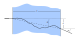
\includegraphics[width=0.9\textwidth]{images/Detector/MultipleScattering.pdf}
    \caption[Schematic View of Multiple Coulomb Scattering]{This is a schematic view of multiple coulomb scattering projected onto a \gls{2d} plane. The solid line is the trace of a particle traversing the detector medium with a thickness $x$, while being deflected by the distance $y$. $\psi$ and $\theta$ denote the deflection angle and scattering angle respectively. This image is sourced from \cite{PDG2018}.}
    \label{fig:MultipleScattering}
\end{figure}
% TODO Maybe move this figure to the end of the paragraph
The \gls{rms} values of these deflection variables in the \gls{2d} plane, $\psi_\text{RMS}$ and $y_\text{RMS}$, are connected to $\theta_\text{RMS}$ and $x$ by \cite{PDG2018}
\begin{align}
    \psi_\text{RMS} &= \frac{1}{\sqrt{3}}\theta_\text{RMS}, \nonumber \\
    y_\text{RMS} &= x \psi_\text{RMS} = \frac{x}{\sqrt{3}}\theta_\text{RMS}.
\end{align}
Since $\theta_\text{RMS}$ is generally rather small, above equation for $y_\text{RMS}$ is simplified, since for small $\theta_\text{RMS}$ we are allowed to replace $\sin{(\theta_\text{RMS})}$ with $\theta_\text{RMS}$. For a momentum measurement in a \gls{lartpc} we observe the random variables within various small columns of \gls{lar} along a particle track. Large deflections are discarded, since they do not contribute to the Gaussian distribution. From this we determine the \gls{rms} variables by a fit over a histogram of the random variables. The column size has to be chosen carefully, because there has to be enough statistics for a $\theta_\text{RMS}$ fit but the column also has to be small enough to avert smearing due to the particle's energy loss. With $\theta_\text{RMS}$ established, it is easy to determine the momentum $p$ by solving equation \ref{eq:MultipleScattering} accordingly. Naturally the multiple scattering method is less accurate than the $\langle -dE/dx \rangle$ measurement. Furthermore, it can not be used for particle identification, since equation \ref{eq:MultipleScattering} only shows a weak particle mass dependence introduced by $\beta$ (consult table \ref{tab:BetheBlochVariables}) which vanishes with high momenta. The MicroBooNE collaboration uses the momentum reconstruction through multiple scattering only for events, whereby the Bragg peak is not contained within the active volume. Given the neutrino beam energy and MicroBooNE's size, these ``uncontained'' tracks are most likely muons.
% TODO ask Davide for the multiple scattering vs. de/dx reconstruction efficiency plots and put it here

A third method to determine a charged particle's momentum could potentially be exploited by the introduction of a strong uniform magnetic field $\vec{B}$ in the active volume. In such a setup, a particle with charge $ze$ and momentum $p = \abs{\vec{p}}$ is subject to the \textbf{Lorentz force} while traversing the magnetic field at a pitch angle $\lambda > \num{0}$. Said pitch angle is defined as the angle between $\vec{p}$ and $\vec{B}$. As the particle looses its momentum in \gls{lar}, its trajectory takes the shape of a spiral with curvature radius $R$ at a given point. In such a case the particle momentum in units of $[\si{\giga\electronvolt}/c]$ is given by \cite{PDG2018}
\begin{equation}
    p = 0.3\, \frac{z R |\vec{B}|}{\cos{(\lambda)}},
\end{equation}
while the units of $|\vec{B}|$ are in $[\si{\tesla}]$ and the units of $R$ in $[\si{\metre}]$. For a momentum measurement in a \gls{lartpc} experiment, one would simply measure the curvature radius $R$ at various points of the track in the upfront calibrated and well known magnetic field. In combination with the outstanding track resolution of a \gls{tpc}, this method would certainly yield the most accurate momentum measurement method, regardless of the track being contained or not. The principle of a working magnetised \gls{lartpc} has already been shown by A. Badertscher \etal \cite{LArTPCMagnetised}, but beyond this small prototype no other experiment has ever used a magnetic field in their active volume. 

In my opinion the persisting reliance on $\langle -dE/dx\rangle$ and $\theta_\text{RMS}$ for momentum measurements marks one of the major shortcomings in our field. We are often blinded by the nice-looking event displays with all their details, forgetting to address the difficulties hidden behind the beauty. The problem could be mitigated by a magnetised \glspl{lartpc}, an idea often proposed, but so far always rejected in the final designs of new detectors. As we reconstruct particle interactions, we eventually rely on hard numbers instead of just beautiful images. Especially for large scale experiments, a magnetised detector should be considered. Unfortunately, magnetised \glspl{lartpc} might not be used in the next generation of large scale detectors.

\section{Energy Dissipation of Neutral Particles} \label{sec:EnergyDissipationNeutral}
Neutral particles, \ie particles without an electric charge, can not be detected directly in a \gls{lartpc}. Their detection depends on a primary interaction which eventually produces charged secondary particles. From these charged secondaries, one tries to reconstruct the neutral particle's energy as well as identifying its flavour. An extreme case of these reconstruction efforts is certainly the neutron, $n$. With a lifetime of ${\tau_n = \SI{880.2(10)}{\second}}$ \cite{PDG2018} it will not decay within a useful time frame for a \gls{lartpc}, since a full \gls{tpc} drift is of the order of milliseconds. Therefore, neutrons can only be detected through spallation events with an argon atom's core, which leave small and localised ionisation spots. Neutron detection, is the major weakness of most noble fluid detectors \cite{NobleGasDetectors}, but there are efforts underway to better reconstruct them. Other neutral hadrons are less problematic, since they decay much faster. The neutral pion $\pi_0$, for instance, features a lifetime of $\tau_{\pi_0} = \SI{8.51(18)e-17}{\second}$ \cite{PDG2018}, after which it most likely decays into two photons. Heavier neutral \glspl{Meson} also feature short lifetimes and decay either into charged particles, lighter neutral \glspl{Meson}, or directly into photons. In the end all neutral \glspl{Meson} eventually leave traces in the detector. Photons, as the force carrier of the \gls{em} force, are a special case and their interaction in \gls{lar} will be described below in more detail.

Of all neutral particles, photons stand out, as they are able to take part in \gls{em} interactions with the detector medium or target material. The photon features three detectable interaction modes in a \gls{lartpc}: \textbf{photoelectric absorption} \cite{PhotoelectricEffect}, \textbf{Compton scattering} \cite{ComptonScattering}, and \textbf{pair production} \cite{PairProduction}, also often referred to as \textbf{photon conversion}. The Feynman diagrams of these processes are depicted in figure \ref{fig:PhotonInteractions}. All three processes are prevalent in different photon energy ranges, depending on the target material. In \gls{lar} the photoelectric absorption is dominant at energies $E \lesssim \SI{0.1}{\mega\electronvolt}$, in the interval $\SI{0.1}{\mega\electronvolt} \lesssim E \lesssim \SI{10}{\mega\electronvolt}$ Compton scattering is prevalent, and at high energies, $E \gtrsim \SI{10}{\mega\electronvolt}$, one finds predominantly pair production (see figure \ref{fig:PhotonAbsorption}). Note, there are two photon interaction channels not listed here, as they are not visible in a \gls{lartpc}. These are: \textbf{photonuclear interactions} \cite{PhotonuclearInteraction} leading to nuclear excitation or fission of heavy elements, if the photon exhibits a respective resonant energy, and \textbf{Rayleigh scattering} \cite{RayleighScattering} which is the elastic form of Compton scattering, \ie the photon does not loose any energy in this process. In the following I will explain the three visible processes with increasing dominance energy.
\begin{figure}[htbp]
    \centering
    \subfloat[Photoelectric Absorption][Photoelectric absorption]
    {
        \fmfframe(10,10)(0,10){\begin{fmfgraph*}(100,50)
            \fmfleft{i1,i2}
            \fmfright{o1,o2}
            \fmf{photon}{i2,v1}
            \fmf{fermion}{i1,v1,v2}
            \fmf{phantom,tension=2}{o1,v2,o2}
            \fmfv{label=$e^-$,label.angle=180,label.dist=0.1cm}{i1}
            \fmfv{label=$\gamma$,label.angle=180,label.dist=0.1cm}{i2}
            \fmfv{label=$e^-$,label.angle=0,label.dist=0.1cm}{v2}
            \fmfv{decor.shape=circle,decor.filled=full,decor.size=1thick}{v1}
        \end{fmfgraph*}}
        \label{fig:PhotoEffect}
    } \hfill
    \subfloat[Compton Scattering][Compton scattering]
    {
        \fmfframe(10,10)(0,10){\begin{fmfgraph*}(100,50)
            \fmfleft{i1,i2}
            \fmfright{o1,o2}
            \fmf{photon}{i2,v1}
            \fmf{photon}{o2,v2}
            \fmf{fermion}{i1,v1,v2,o1}
            \fmfv{label=$\gamma$,label.angle=180,label.dist=0.1cm}{i2}
            \fmfv{label=$e^-$,label.angle=180,label.dist=0.1cm}{i1}
            \fmfv{label=$e^-$,label.angle=0,label.dist=0.1cm}{o1}
            \fmfv{label=$\gamma$,label.angle=0,label.dist=0.1cm}{o2}
            \fmfv{decor.shape=circle,decor.filled=full,decor.size=1thick}{v1}
            \fmfv{decor.shape=circle,decor.filled=full,decor.size=1thick}{v2}
        \end{fmfgraph*}}
        \label{fig:ComptonScattering}
    } \hfill
    \subfloat[Pair Production][Pair production]
    {
        \fmfframe(10,10)(0,10){\begin{fmfgraph*}(100,50)
            \fmfleft{i1,i2}
            \fmfright{o1,o2}
            \fmf{photon,label=$\gamma$,label.side=left,label.dist=0.1cm}{i1,v1}
            \fmf{photon}{i2,v2}
            \fmf{fermion}{o2,v2,v1,o1}
            \fmfv{label=$Z$,label.angle=180,label.dist=0.0cm,decor.shape=circle,decor.filled=30,decor.size=8thick}{i1}
            \fmfv{label=$\gamma$,label.angle=180,label.dist=0.1cm}{i2}
            \fmfv{label=$e^-$,label.angle=0,label.dist=0.1cm}{o1}
            \fmfv{label=$e^+$,label.angle=0,label.dist=0.1cm}{o2}
            \fmfv{decor.shape=circle,decor.filled=full,decor.size=1thick}{v1}
            \fmfv{decor.shape=circle,decor.filled=full,decor.size=1thick}{v2}
        \end{fmfgraph*}}
        \label{fig:PairProduction}
    }
    \caption[Feynman Diagrams of the Photon Interaction Modes]{Shown here are the Feynman diagrams of the three photon interaction modes with the atomic shell of a detector medium. In all three diagrams the incident photon, denoted as $\gamma$, is depicted in the upper left corner. The photoelectric absorption is shown in \subref{fig:PhotoEffect}, Compton scattering in \subref{fig:ComptonScattering}, and pair production in \subref{fig:PairProduction}. The spectator of the pair production process is usually an atomic nucleus and thus depicted above as a grey blob labelled with the atomic number $Z$ of the target atom. Note that the spectator could also be an electron.}
    \label{fig:PhotonInteractions}
\end{figure}
During the photoelectric absorption, shown in figure \ref{fig:PhotoEffect}, the incident photon is absorbed and its full energy transferred to an electron in the atomic shell of the target material. While undergoing Compton scattering, shown in figure \ref{fig:ComptonScattering}, the photon only conveys a part of its energy to a shell electron and thereafter is able to interact further. Usually several Compton scattering processes occur before the photon has lost enough energy and is ultimately absorbed photoelectrically. During pair production, as shown in figure \ref{fig:PairProduction}, the photon is converted into an electron-positron pair, wherefore it has to exhibit an initial energy of at least twice the electron mass, \ie $E_\gamma \geq 2 m_e c^2 = \SI{1.022}{\mega\electronvolt}$. Below said threshold, no conversion can occur. Since pair production by a single photon is violating momentum conservation in some reference frames, a spectator has to present, exchanging an additional photon. The spectator of the pair production process is usually an atomic nucleus, in about \SI{95}{\percent} of the cases in \gls{lar}. In the other $\sim \SI{5}{\percent}$ of the pair production events, the spectator is an electron (see figure \ref{fig:PhotonAbsorption}). As can be seen, eventually every photon is either converted into - or looses its energy to charged particles, which are then detectable in a \gls{lartpc}. 

When considering photon interactions in matter, they are mostly characterised by their intensity as a function of distance travelled in a medium $I(x)$. Said intensity is defined as
\begin{equation} \label{eq:PhotonAttenuation}
    I(x) = I_0 e^{-\mu x},
\end{equation}
with the initial intensity, $I_0$, and the attenuation coefficient, $\mu$, in units of $[\si{\per\centi\metre}]$. The whole term $\exp(-\mu x)$ actually denotes the absorption probability for a single photon. Thus, $I(x)$ of above equation is a statistical distribution and does not determine a single photon's fate, similar to $\langle -dE/dx\rangle$. Furthermore, $\mu$ is actually a function of the photon's initial energy, as shown in figure \ref{fig:PhotonAbsorption}.
\begin{figure}[htbp]
    \centering
    \includegraphics[width=0.9\textwidth]{images/Detector/PhotonAbsorption.pdf}
    \caption[Attenuation Coefficient of Photons in Liquid Argon as a Function of Energy]{Shown here is the attenuation coefficient of photons, $\mu$, in \gls{lar} as a function of photon energy $E$. At energies $E \lesssim \SI{0.1}{\mega\electronvolt}$ the energy dissipation of photons is dominated by photoelectric absorption, in the interval $\SI{0.1}{\mega\electronvolt} \lesssim E \lesssim \SI{10}{\mega\electronvolt}$ by Compton scattering, and at high energies $E \gtrsim \SI{10}{\mega\electronvolt}$ by pair production. For $E \gtrsim \SI{1}{\giga\electronvolt}$, $\mu$ becomes a constant defined by the radiation length, \ie $\mu = 7\rho/(9X_0)$. The data presented in this chart is provided by XCOM \cite{LArPhotonAbsorption}.}
    \label{fig:PhotonAbsorption}
\end{figure}
As can be seen in said graph, the three photon interaction modes contribute in different energy intervals. Furthermore, the \textbf{pair production} is split up into its two components: the interaction in the nuclear field in dark blue and the interaction in the electron field in light blue. In \gls{lar} at photon energies of $E \gtrsim \SI{1}{\giga\electronvolt}$, the absorption coefficient becomes constant and can be written as
\begin{equation}
    \mu(E > \SI{1}{\giga\electronvolt}) = \frac{7}{9}\frac{\rho}{X_0},
\end{equation}
with $\rho$ representing the \gls{lar} density and $X_0$ the radiation length, as previously introduced in equation \ref{eq:Bremsstrahlung}. As a reminder, we defined $X_0$ by the mean distance $X_0/\rho$ over which an electron loses all but $1/e$ of its energy by Bremsstrahlung. Often, the free mean path, $\lambda$, of a photon is used in above considerations instead of $\mu$, it is defined as $\lambda = 1/\mu$. Thus we get the second definition for $X_0$: the distance $X_0/\rho$ represents $7/9$ of the free mean path of pair production by a high energy photon, $\lambda_\text{p.p}$ \cite{PDG2018}. This ought to show how closely related electron and photon interactions are. So how do we actually determine photon energies in a \gls{lartpc}? With the photon absorption, we are again facing random processes, but sometimes they only occur once per photon, unlike ionisation or multiple Coulomb scattering. The solution for this problem is \gls{em} shower reconstruction. 

By now we established that a photon eventually looses its energy to electrons and positrons, through the interaction modes shown in figure \ref{fig:PhotonInteractions}, but the chain of interactions does not end with these secondary particles loosing their energy by ionisation. As shown in section \ref{sec:ParticleInteractions}, especially in figure \ref{fig:BetheBloch}, light particles are dominated by radiative energy losses already at relatively low energies, \ie they exhibit a low critical energy $E_\text{c}$. For electrons and positrons radiative losses are dominant for $E \gtrsim \SI{32}{\mega\electronvolt}$. As the name implies photons are emitted through Bremsstrahlung, during said radiative losses. In the case of the positron, annihilation has to be considered as well, since it is an antimatter particle. The Feynman diagrams of the Bremsstrahlung and electron-positron annihilation \cite{ElectronPositronAnnihilation1,ElectronPositronAnnihilation2} processes are shown in figure \ref{fig:ElectronPositronInteractions}.
\begin{figure}[htbp]
    \centering
    \subfloat[Bremsstrahlung][Bremsstrahlung]
    {
        \fmfframe(10,10)(0,10){\begin{fmfgraph*}(120,60)
            \fmfleft{i1,i2}
            \fmfright{o1,o2}
            \fmf{phantom,tension=2}{i1,v1,i2}
            \fmf{photon}{v2,o2}
            \fmf{fermion}{v1,v2,o1}
            \fmfv{label=$e^\pm$,label.angle=180,label.dist=0.1cm}{v1}
            \fmfv{label=$e^\pm$,label.angle=0,label.dist=0.1cm}{o1}
            \fmfv{label=$\gamma$,label.angle=0,label.dist=0.1cm}{o2}
            \fmfv{decor.shape=circle,decor.filled=full,decor.size=1thick}{v2}
        \end{fmfgraph*}}
        \label{fig:Bremsstrahlung}
    } \qquad \qquad
    \subfloat[Electron-Positron Annihilation][Electron-positron annihilation]
    {
        \fmfframe(10,10)(0,10){\begin{fmfgraph*}(120,60)
            \fmfleft{i1,i2}
            \fmfright{o1,o2}
            \fmf{photon}{v1,o1}
            \fmf{photon}{v2,o2}
            \fmf{fermion}{i1,v1,v2,i2}
            \fmfv{label=$e^-$,label.angle=180,label.dist=0.1cm}{i1}
            \fmfv{label=$e^+$,label.angle=180,label.dist=0.1cm}{i2}
            \fmfv{label=$\gamma$,label.angle=0,label.dist=0.1cm}{o1}
            \fmfv{label=$\gamma$,label.angle=0,label.dist=0.1cm}{o2}
            \fmfv{decor.shape=circle,decor.filled=full,decor.size=1thick}{v1}
            \fmfv{decor.shape=circle,decor.filled=full,decor.size=1thick}{v2}
        \end{fmfgraph*}}
        \label{fig:ElectronPositronAnnihilation}
    }
    \caption[Feynman Diagrams of the Electron and Positron Interaction Modes in an EM Shower]{Shown here are the Feynman diagrams of the electron and positron interaction modes in an \gls{em} shower. An important interaction mode missing here is ionisation, which is depicted in figure \ref{fig:IonisationAndExcitation}.}
    \label{fig:ElectronPositronInteractions}
\end{figure}
Both depicted processes produce at least one additional photon after a mean distance of $X_0/\rho$. This photon will again be able to produce electrons and positrons after a mean distance of $\lambda_\text{p.p} = 9X_0/(7\rho)$, if its energy is high enough. This leads to a cascade of secondary particles called shower. Such an \gls{em} shower could principally be induced by either an electron or a photon as a primary particle.
% TODO Maybe show a picture of a shower in uBooNE
Futhermore, these \gls{em} showers show several useful universal properties, which massively simplify their reconstruction. For instance, there is the \textbf{Moli\`ere radius} $R_\text{m}$ given by \cite{MoliereRadius}
\begin{equation}
    R_\text{m} = X_0 \, \frac{\SI{21.2}{\mega\electronvolt}}{E_\text{c}}.
\end{equation}
It defines the radius of a cylinder along the shower axis within which \SI{90}{\percent} of the initial particle's energy is dissipated. Within a radius of $2R_\text{m}$, \SI{95}{\percent} of the energy is contained. Since the radius of said cylinder is only material dependent and otherwise constant for all energies of the initial shower particle, it becomes obvious that the length of the shower has to exhibit an energy dependence. Said shower length, $X$, is defined by the following relation \cite{ExperimentalTechniques}
\begin{equation}
    X = X_0 \left( \ln{\left(\frac{E}{E_\text{c}}\right)} + C_j \right), \qquad \text{with} \ C_j =
    \begin{cases}
        -1.0 & \text{for} \ j=e^- \\
        -0.5 & \text{for} \ j=\gamma
    \end{cases},
\end{equation}
where $j$ denotes the initial particle flavour inducing the shower. Above equation can thus be used to directly calculate the energy of an initial particle of an \gls{em} shower. However, for any shower energy reconstruction to work, the whole shower has to be contained in the active volume. One question that remains open now is: how do we distinguish the initial particles? The answer is quite simple, it is done through the linear stopping power at the starting point of the shower. If $j = e^-$, we expect a track with a mean length of $X_0$ before the shower starts. On this track we expect $\langle -dE/dx\rangle \approx \langle -dE/dx\rangle_\text{MIP}$. If, however, $j = \gamma$, we expect two tracks and thus a linear stopping power of $\langle -dE/dx\rangle \approx 2 \langle -dE/dx\rangle_\text{MIP}$. This calorimetric discrimination of electron and photon showers marks one of the strengths of the \gls{lartpc} technology, due to its excellent $\langle -dE/dx\rangle_\text{ion}$ and spacial resolutions. An example of said discrimination in a \gls{lartpc} is shown in figure \ref{fig:ElectronPhotonDiscrimination} below.
\begin{figure}[htbp]
    \centering
    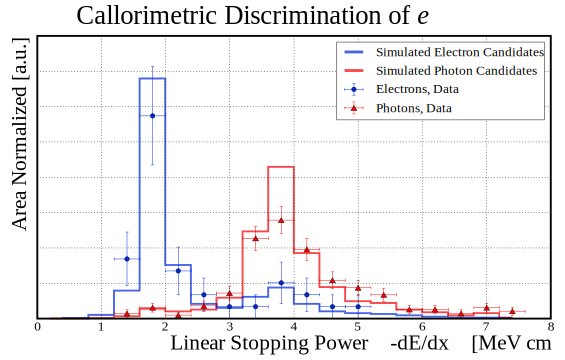
\includegraphics[width=0.8\textwidth]{images/Detector/ElectronPhotonDiscrimination.pdf}
    \caption[Calorimetric Discrimination of Electrons and Photons in a LArTPC]{Calorimetric discrimination of electrons and photons in a \gls{lartpc}, here the results of the ArgoNeuT experiment \cite{LArTPCElectronPhotonDiscrimination}.}
    \label{fig:ElectronPhotonDiscrimination}
\end{figure}
This figure shows a prominent peak at $\langle -dE/dx\rangle = \langle -dE/dx\rangle_\text{MIP}$ for electron induced showers and a slightly broader peak at $\langle -dE/dx\rangle = 2\langle -dE/dx\rangle_\text{MIP}$ for photon induced showers. However, it also becomes apparent that said electron-photon discrimination method is not perfect. It still relies on random processes like the $\langle -dE/dx\rangle$ measurement in a short distance as well as the photon interaction probability $\exp (-\mu x)$. Furthermore, there is the possibility of asymmetric energy allocation to the positron and the electron during pair production. The latter contributes to the broadening of the photon peak to lower $\langle -dE/dx\rangle$. Also, a photon can simply produce a high energy Compton electron creating a \gls{em} shower, which explains the small peak around $\langle -dE/dx\rangle = \langle -dE/dx\rangle_\text{MIP}$ in the photon channel. When the cascade starts to develop in the probing distance of $\langle -dE/dx\rangle_\text{ion}$, higher than expected linear stopping powers are registered.

In the case of MicroBooNE, this excellent calorimetric discrimination between photons and electrons was the main reason for choosing the \gls{lartpc} technology (see MicroBooNE proposals \cite{MicroBooNEProposal1, MicroBooNEProposal2}). The idea being the reduction of the massive \mbox{$\pi_0 \to \gamma + \gamma$} background experienced during MiniBooNE's \gls{lee} measurement. Since MiniBooNE is a Cherenkov detector, it is merely impossible to differentiate between photon and electron induced showers. The reduced background in MicroBooNE is expected to either increase the certainty level of the respective \gls{lee} measurement to $7\sigma$ or reject MiniBooNE's findings.
% TODO Make reference to MiniBooNE result in theory (comming up)

\section{Multiphoton Ionisation by UV-Laser} \label{sec:MultiPhotonIonisation}
A method to ionise \gls{lar} in a controlled manner can be introduced by the use of a coherent beam of photons, a laser. They offer straight ionisation paths with uniform energy deposition along it, creating standard tracks ideal for detector calibration. In principle one could ionise \gls{lar} by a single photon if its energy $h\nu$ equals or exceeds the ionisation potential, \ie $h\nu \geq I_\text{LAr}$. This implies a photon wavelength of $\lambda \geq \SI{92.5}{\nano\metre}$, but lasers emitting these short wavelengths are not available. However, there is a way to ionise \gls{lar} with a laser, namely multiphoton ionisation \cite{MultiphotonProcesses1,MultiphotonProcesses2}. As the name states, the general working principle of this process is the absorption of multiple photons by a single electron in atomic shell, thereby ionising the argon atom. Energy wise all multiphoton ionisation processes feature a single photon energy smaller than the ionisation potential of the medium, \ie $h\nu < I_\text{LAr}$. Nevertheless multiple photons still fulfil the ionisation criterion, \ie $N h\nu \geq I_\text{LAr}$ with the integer $N$ denoting the number of photons. The prove of concept of multiphoton ionisation in \gls{lar} was achieved by J. Sun \etal \cite{LArLaserFirst}. Later our \gls{lar} group at the \gls{lhep} of the University of Bern refined the technology by adding beam energy control, making the technology viable for calibration use cases \cite{LArLaserLHEP}. In the following paragraphs, I will determine the conditions for a multiphoton absorption to occur in \gls{lar}.

We distinguish between three different multiphoton processes: the resonant, the quasi-resonant, and the non-resonant (direct) multiphoton ionisation. In the resonant case the energy of at least one photon equals the energy of a bound excited state with index $i$, \ie $N h\nu = E_i$. These states are relatively long-lived with a lifetime of $\tau_\text{res} \approx \SI{e-8}{s}$ \cite{MultiphotonProcesses1}. However, a purely resonant multiphoton absorption is experimentally hard to achieve, since it would require light beams of different wavelengths to be perfectly aligned and to be fired within the $\tau_\text{res}$ time frame. It thus is favourable to use a single, monochromatic light source. Still, resonant multiphoton absorption plays an important role for most applications, as we will see later.

As their names imply, quasi-resonant and non-resonant multiphoton inonisation occure through virtual states, which are not eigenstates of the atom. In the quasi-resonant case, however, said virtual state is close and slightly above an excited bound state. The non-resonant ionisation does not require any intermediate atomic states. This is possible due to the uncertainty principle first postulated by W. Heisenberg \cite{UncertaintyPrinciple}. In the energy and time realm it can be written as $\Delta E \Delta t \geq \hbar/2$, meaning that the product of the uncertainty in energy $\Delta E$ of an atomic state and the time interval of its existence $\Delta t$ are greater or equal than $\hbar/2$. This relation also defines the lifetime of these virtual states \cite{MultiphotonProcesses1}
\begin{equation} \label{eq:VirtualStateLifetime}
    \tau_\text{virt} = \frac{\hbar}{\Delta E}.
\end{equation}
For the quasi-resonant states $\Delta E$ is directly given by the difference between its energy $E_\text{qr}$ and the next lower atomic state $E_i$, \ie $\Delta E = E_\text{qr} - E_i$. In case of non-resonant states $\Delta E$ is simply the energy difference between the atomic state (mostly the ground state) and the virtual state $\Delta E = N h \nu$. As an example let us consider single photon virtual state ($N=1$) with a wavelength of $\lambda = \SI{266}{\nano\metre}$ exciting a ground state electron to a virtual state. Said virtual state would exhibit a life time of only $\tau_\text{virt} = \SI{1.4e-16}{\second}$, eight orders of magnitude lower than $\tau_\text{res}$. Thus the light source needs to provide a high optical intensity as well as a high level of spacial and temporal coherence in order to induce multiple interactions within this short time frame, properties only found in lasers.

Before we are able to introduce the physical quantities which describe multiphoton processes, we first need to establish some basic formulas of laser physics. For commercially available pulsed lasers key values like pulse width, pulse energy, and wavelength (photon energy) are provided by the manufacturer. From these we can deduce the optical power of a single pulse $P$ as \cite{LaserBasics2}
\begin{equation} \label{eq:PulsePower}
    P = f \frac{E_\text{p}}{\tau_\text{p}},
\end{equation}
where $E_\text{p}$ denotes the pulse energy, $\tau_\text{p}$ the pulse width, and $f$ the pulse shape factor with $f \approx \num{0.94}$ for a Gaussian pulse in time. For reasons of simplification we often consider a Gaussian intensity profile along the beam radius $r$, \ie a so-called \textbf{Gaussian beam}. Thus the intensity is given by \cite{LaserBasics1}
\begin{equation} \label{eq:OptialIntensity}
    I(r) = I_0 e^{-\frac{2r^2}{w^2}}, \quad \text{with} \quad I_0 = \frac{2P}{\pi w^2}.
    % TODO introduce z-dependency with w(z)
\end{equation}
with $w$ standing for the beam diameter, which itself is variable along the beam axis. Using $I_0$ we can calculate the electric field strength amplitude of the laser beam \cite{MultiphotonProcesses2}
\begin{equation} \label{eq:LaserFieldStrength}
    F = \sqrt{\frac{2I_0}{c\epsilon_0\epsilon_\text{r}}}.
\end{equation}

With these quantities established, we are now ready to introduce the main quantity influencing the appearance of multiphoton ionisation, which is the multiphoton ionisation rate per single target molecule, as \cite{MultiphotonProcesses1,MultiphotonProcesses2}
\begin{equation} \label{eq:MultiphotonRate}
    W = \sigma^{(N)} \Phi_\text{ph}^N = \sigma^{(N)} \left(\frac{I}{h\nu} \right)^N.
\end{equation}
Above equation features the generalised cross section of the multiphoton ionisation process $\sigma^{(N)}$ of the $N$\textsuperscript{th} order (units: $[\sigma^{(N)}] = [\si{\centi\metre\tothe{2N}\second\tothe{N-1}}]$), with $N$ again denoting the number of photons necessary to surpass the ionisation potential. Furthermore, we used the photon flux $\Phi_\text{ph}$ given by the intensity of the laser beam $I$ and the single photon energy $h\nu$. Above formula shows the importance of the intensity, since the rate grows with $I^N$. The cross section, though, diminishes rapidly with increasing order, which becomes obvious when considering the process of multiphoton absorption. The first photon excitation to a virtual state features the first order cross section $\sigma^{(1)}$, which has a relatively high value, since there are plenty of stable ground states for a photon to interact with. For the absorption process of a second photon by this first virtual state, the cross section is truncated by the short lifetime and the density of said states in that medium. The two-photon cross section $\sigma^{(2)}$ is therefore the product of $\sigma^{(1)}$ and the cross section of the interaction of a second photon. In summary, it can be stated, that with every additional non-resonant ionisation step, an ever smaller cross section gets multiplied to the previous one, \eg typically resulting in $\sigma^{(1)} \sim \SI{e-17}{\centi\metre\squared}$, $\sigma^{(2)} \sim \SI{e-49}{\centi\metre\tothe{4}\second}$, $\sigma^{(3)} \sim \SI{e-81}{\centi\metre\tothe{4}\second}$, \etc in non-resonant cases \cite{MultiphotonProcesses1}. However, this statement is not valid if resonant states are involved, as is the case in \gls{lar}. For beam intensities higher than \SI{100}{\kilo\watt\per\centi\metre\squared} the ionisation rate of a resonant state is much greater than its decay rate to the ground state, thus greatly increasing $\sigma^{(N)}$ \cite{MultiphotonProcesses1}.

There is, however, another criterion our system needs to fulfil in order to allow the use of the ionisation rate formula in equation \ref{eq:MultiphotonRate}. It is introduced through the adiabatic parameter $\gamma$ for a laser beam in \gls{lar} \cite{MultiphotonCriterion}
\begin{equation}
    \gamma = \omega \frac{\sqrt{2m_eI_\text{LAr}}}{eF}.
\end{equation}
We now can use $\gamma$ to establish the criterion for multiphoton absorption to occur as $\gamma^2 \gg 1$. If $\gamma^2 \ll 1$ the ionisation would be dominated by the tunnel effect, whereby the electron is able to pass through the potential barrier of the atom which is strongly warped by the high electric field strength of the laser beam. When using the values form the first section of table \ref{tab:LaserProperties} for MicroBooNE's laser calibration system as an example, we get $P = \SI{9.4(2)}{\mega\watt}$, $I_0 = \SI{16.6(4)}{\mega\watt\per\centi\metre}$, and thus $F = \SI{91.3(21)}{\kilo\volt\per\centi\metre}$. This results in a $\gamma^2 = \num{5.73e26}$, which clearly meets the condition of $\gamma^2 \gg 1$ and we conclude that typical commercially available lasers are subject to multiphoton absorption in \gls{lar}. In order to be in the realm of tunnel effect dominance, much more powerful lasers would be required than the one of our example.

With an ionisation potential in \gls{lar}, $I_\text{LAr} = \SI{13.4}{\electronvolt}$, and a laser with a wave length of $\lambda = \SI{266}{\nano\metre}$ or a photon energy of $h\nu = \SI{4.66}{\electronvolt}$, a total of three photons are necessary to induce a multiphoton ionisation process, \ie $N = \num{3}$ and thus $Nh\nu = \SI{13.89}{\electronvolt}$. In order to understand the characteristics of this three-photon absorption in \gls{lar} we need to again consider the energy bands of figure \ref{fig:ArEnergyLevelsLiquid}. The first ionisation stage at \SI{4.66}{\electronvolt} is non-resonant, with the aforementioned lifetime of $\tau_\text{virt} = \SI{1.4e-16}{\second}$. The second photon at \SI{9.32}{\electronvolt}, though, seems to fall into several bands and the transition might thus be resonant. But first we have to check if it is an allowed transition. A single photon exhibits two total angular momentum states $J = \pm 1$ given purely by its spin \cite{PDG2018}. Therefore two photons interacting with an single electron are able to change its angular momentum by $\Delta J = -2,0,+2$. Considering argon's ground state with an electron configuration of $1s^2 2s^2 2p^6 3s^2 3p^6$ with $J = 0$ \cite{ArgonEnergyLevels2} and the fact that there are no negative total angular momentum states, it follows that only resonant transition with $J = 0,2$ are allowed. In figure \ref{fig:ArEnergyLevelsLiquid}, the \gls{lar} band structure of excited states with $J = 0,2$ is shown including the three-photon absorption levels. From this we deduce that only two bands are close to the two-photon energy level at \SI{9.32}{\electronvolt}. The first and lower energy state is $1s^2 2s^2 2p^6 3s^2 3p^5\ch{(^2P_{3/2}^o)}4s$ with $J = 2$ \cite{ArgonEnergyLevels2}, which has an upper band boundary of \SI{9.26}{\electronvolt} and thus falls in the quasi-resonant category. This particular quasi-resonant state has a life time of $\tau = \SI{4.3e-13}{\second}$ before decaying into the resonant state. However, since the energy of the third photon still suffices to ionise the atom from said resonant state on, we can consider it as a resonant process for two photons with combined $J = 2$. The band of the second atomic excited state $1s^2 2s^2 2p^6 3s^2 3p^5\ch{(^2P_{1/2}^o)}4s$ with $J = 0$ \cite{ArgonEnergyLevels2} is located between \SIrange{9.28}{9.44}{\electronvolt} and hence is in resonance with a two-photon absorption with a combined angular momentum of $J = 0$. Finally the third and last photon is able to ionise the argon atom in both cases.
\begin{figure}[htbp]
    \centering
    \includegraphics[width=0.6\textwidth]{images/Detector/ArEnergyLevelsLaser.pdf}
    \caption[UV-Laser Induced Three-Photon Ionisation in LAr]{This graph shows the \gls{uv}-laser induced three-photon ionisation process in \gls{lar}. The \gls{uv}-laser in question has a wave length of \SI{266}{\nano\metre} or a photon energy of \SI{4.66}{\nano\metre}, resulting in a three-photon ionisation process with levels at \SIlist{4.66;9.32;13.98}{\electronvolt} drawn in purple. Represented by blue bands are all excited atomic states with a total angular momentum of $J = 0$ and in green the ones with $J=2$ (extracted from figure \ref{fig:ArEnergyLevelsLiquid}). The first ionisation stage is non-resonant, however, the second exhibits a resonance with the band structure of the excited states in \gls{lar} for a combined angular momentum of both photons involved of $J = 0$ ($3p^5\ch{(^2P_{1/2}^o)}4s$), as well as a quasi-resonance for $J = 2$ ($3p^5\ch{(^2P_{3/2}^o)}4s$) \cite{ArgonEnergyLevels2}. From these resonant states the third photon is then able to ionise the excited argon atom by a comfortable margin.}
    \label{fig:ArEnergyLevelsLaser}
\end{figure}

Due to the aforementioned resonance after two photon stages in \gls{lar}, the three-photon ionisation cross section $\sigma^{(3)}$ is a product of the two-photon cross section $\sigma^{(2)}$ and the cross section of a single photon ionising the atom from said bound resonant state $\sigma^{(1)}_{\text{res}}$, \ie $\sigma^{(3)} = \sigma^{(2)} \sigma^{(1)}_{\text{res}}$. The only cross section measurement in \gls{lar}, using the same laser type as MicroBooNE (see section \ref{sec:LaserCalibrationSystem}), was performed by the Argontube group at \gls{lhep} in 2010 \cite{LArLaserCrossSection}. Back then they found that $N = \num{2.02(5)}$ by fitting the three-photon ionisation rate of equation \ref{eq:MultiphotonRate} as a function of photon flux $\Phi_\text{ph}$. This means that the ionisation probability from the resonant state onward is close to one for the laser intensities used in \glspl{lartpc}. Thus our three-photon process of \SI{266}{\nano\metre} photons in \gls{lar} becomes a two-photon process with a cross section measured as \cite{LArLaserCrossSection}
\begin{equation}
    \sigma^{(2)}_{\text{LAr}} = \SI[parse-numbers=false]{\left( 1.24 \pm 0.10_\text{stat} \pm 0.30_\text{syst}\right)\times 10^{-56}}{\centi\metre\tothe{4}\second}.
\end{equation}
Again using MicroBooNE's laser system as an example (see table \ref{tab:LaserProperties}), we get an ionisation rate per argon atom in the laser beam of $W = \SI{6.14e-6}{\per\second}$ resulting in an ionisation yield of roughly \SI{2000}{\per\milli\metre} in the laser track (I checked this number tenfold, cross section is indeed way too low. There is no way this cross section number is supported by the data, must be a calculation error (unit conversion or something)).

% Kerr effect
Another phenomenon influencing the multiphoton ionisation by laser is the Kerr effect. It describes the shift of the refractive index $\Delta n$ of a medium which is subject to high electric fields $E$ \cite{KerrEffect}. Said shift appears due to the induced dielectric polarisation of the material. In static electric fields the effect can be described as
\begin{equation}
    \Delta n = K \lambda E^2,
\end{equation}
with $K$ denoting the material dependent Kerr constant and $\lambda$ the wave length of the refracted light. The Kerr effect can also be induced by dynamic fields, \eg high intensity laser beams with $I > \SI{100}{\kilo\watt\per\centi\metre\squared}$ \cite{KerrEffectLaser}, and is then called \textbf{optically induced Kerr effect}. In this case the shift in refractive index becomes beam intensity dependent and can be approximated by \cite{LaserTheory}
\begin{equation}
    \Delta n \approx n_2 I(r).
\end{equation}
Here, $n_2$ stands for the material dependent nonlinear index of refraction and $I(r)$ for the optical intensity. When considering a idealised laser beam with a Gaussian intensity profile along its radius $r$ (see equation \ref{eq:OptialIntensity}), it follows that $\Delta n$ also exhibits a Gaussian distribution with a maximum on the beam axis. If the optical intensity is high enough, said radial dependency forms a so-called Kerr lens and the beam is subject to self-focusing \cite{LaserBasics2}.

In \gls{lar} this self-focusing of a high intensity laser beam evokes clusters of increased ionisation along the beam axis which are able to saturate or even damage the readout electronics. It creates also massive amounts of space charge leading to field distortions. Self-focusing was observed many times by the Argontube group, although we never further investigated the effect nor published its observation, so it is badly documented in our field. In order to mitigate self-focusing, the beam intensity is reduced by an optical attenuator, which will be discussed later in this chapter (see section \ref{sec:LaserCalibrationSystem}). The goal is to strike a balance between preventing self-focusing and providing enough optical power in order to still induce three-photon ionisation.
% TODO make glossary entries about multiphoton processes and absorption

\section{Recombination and Scintillation} \label{sec:RecombAndScint}
Now let us go back to the detector medium and follow the processes occurring after particle interactions. Immediately after the ionisation and excitation processes in \gls{lar}, see equations \ref{eq:IonisationProcess} and \ref{eq:ExcitationProcess} respectively, we are left with \glspl{quasifreeelectron} $e^-$, argon ions \ce{Ar^+} and argon \textbf{excitons} \ch{Ar^*}. Then, within a time frame of the order of \SI{e-12}{\second}, argon ions undergo \gls{selftrapping} with one of its neighbouring argon atoms, forming charged argon dimers \ch{Ar2^+} \cite{LArSelf-Trapping},
\begin{equation} \label{eq:SelfTrapping}
    \ce{Ar^+ + Ar ->  \ch{Ar2^+}}.
\end{equation}
Some of these charged dimers then recombine with \glspl{quasifreeelectron}. Note, that this recombination process is dependent on the energy deposited in the medium and how much of said energy is transferred to the \glspl{quasifreeelectron}. In the case of multiphoton ionisation by a laser, for instance, recombination can be neglected \cite{LArLaserCrossSection}. In general, the recombination process proceeds in several stages, as described in \cite{NobleGasDetectorsBetter,LArRecombination}. Initially, the dimer is split up again forming a highly excited state \ch{Ar^{**}},
\begin{equation}
    \ce{\ch{Ar2^+} + $e^-$ -> \ch{Ar^{**}} + Ar}.
\end{equation}
Said highly excited state then decays into an argon \textbf{exciton} \ch{Ar^*} in a non-radiative collision process with other argon atoms,
\begin{equation}
    \ce{\ch{Ar^{**}} + Ar -> \ch{Ar^*} + Ar + \text{heat}}.
\end{equation}
Naturally, these excited argon states \ch{Ar^*} are not only produced through recombination alone, but also directly by the incident particles if the transferred energy is too low to overcome the Coulomb-potential of the atom. The latter \ch{Ar^*} production channel was already established in equation \ref{eq:ExcitationProcess}. In dense argon, with number densities $n > \SI{e19}{\per\centi\metre\cubed}$, these \ch{Ar^*} react in a triple collision with two ground state atoms into an excited dimer state, called \glspl{excimer} \cite{LArSelf-Trapping},
\begin{equation} \label{eq:ExcimerProduction}
    \ce{\ch{Ar^*} + 2Ar ->  \ch{Ar2^*} + Ar}.
\end{equation}
Above described production of \ch{Ar2^*} states is achieved by the process of \gls{dynamicaltrapping}, which is estimated to occur within \SI{6e-12}{\second} after the formation of \ch{Ar^*} \cite{LArSelf-Trapping}. Given the number density of \gls{lar} at its \gls{bp}, $n_\text{LAr} = \SI{2.1e22}{\per\centi\metre\cubed}$, and the life time of \ch{Ar^*} in the range of \SIrange{e-9}{e-7}{\second} \cite{NobleGasDetectors}, the vast majority of \textbf{excitons} in a \gls{lartpc} take the form of \glspl{excimer}, \ch{Ar2^*}. It is these \glspl{excimer}, or rather their chemical decomposition, which are responsible for producing a luminescence called \textbf{scintillation light} described by the following process:
\begin{equation}
    \ce{\ch{Ar2^*} ->  2Ar + $\gamma$}.
\end{equation}
This de-excitation marks the end of the recombination process and will be discussed in more detail in the course of this section.

In a \gls{lartpc}, recombination is suppressed by a drift electric field $\vec{E}$ by pulling the two conversely charged ionisation products apart. Thus the more we increase the field strength, $\vert\vec{E}\vert$, the less recombination will occur. In this context, the ratio $Q/Q_0$ is a useful number to quantify recombination or charge reduction processes in general. With $Q_0$ denoting the total electron charge produced during ionisation and $Q$ the charge left charge reduction process, \ie recombination in this case. The breakthrough in quantifying the behaviour of the charge ratio $Q/Q_0$ as a function of electric field came with the theory of G. Jaff\'e \cite{LArRecombinationModel1}. He was the first to realise that recombination has to be treated within the whole charge column of ionisation track and not just as individually insulated electron-ion pairs. The Jaff\'e model results in charge ratio of
\begin{equation} \label{eq:JaffeModel}
    \frac{Q}{Q_0} = \frac{1}{1+q_0 f\left(\vert \vec{E} \vert \sin{(\phi)}\right)},
\end{equation}
where $q_0$ is the initial density of electron-ion pairs and $f$ is a numerically solvable function depending on the projection of electric field strength to the ionisation track direction $\vert \vec{E} \vert \sin(\phi)$, \ie $\phi$ denotes the angle between the ionisation track and the electric field vector. Furthermore, the Jaff\'e model assumes the electrons and ions to be equally mobile, \ie they move with the same velocity when subject to an electric field. As we will see later in this chapter, the latter assumption is wrong. Thus, J. Thomas and D.A. Imel introduced the box model \cite{LArRecombinationModel2}. It is based on the Jaff\'e model, but presumes stationary ions and mobile electrons while disregarding diffusion effects. Then the electron-ion pairs are isolated and uniformly placed in a cubical box as an initial condition. Due to these assumptions the differential equations introduced by Jaff\'e can be solved analytically, which results in
\begin{equation} \label{eq:BoxModel}
    \frac{Q}{Q_0} = \frac{1}{\xi} \ln \left( 1 + \xi \right), \qquad \xi =  \eta \, \frac{Q_0}{\vert\vec{E}\vert},
\end{equation}
with $\eta$ denoting a free parameter used to fit this model to data points. In conclusion, if $\vert\vec{E}\vert \to \infty$, \ie $\xi \to 0$, there will be no recombination, while with $\vert\vec{E}\vert \to 0$, \ie $\xi \to \infty$, all electron-ion pairs recombine. Another way to fit the Jaff\'e model of equation \ref{eq:JaffeModel} directly is given by Birks' law \cite{LArRecombinationModel3}, resulting in
\begin{equation} \label{eq:BirksLaw}
    \frac{Q}{Q_0} = \frac{1}{1+\frac{k_E}{\vert \vec{E} \vert} }.
\end{equation}
Here $k_E$ is the fit parameter. Today, every experiment uses their own adaptations, either of the box model or the Birks' law simplification of the Jaff\'e model in order to fit them to their respective data. The ICARUS collaboration, for instance, used the following adaptation of the Jaff\'e model and Birks' law \cite{LArRecombinationFunction}:
\begin{equation} \label{eq:RecombinationFunction}
    \frac{Q}{Q_0} = \frac{A}{1+\frac{k}{\vert \vec{E} \vert} \frac{1}{\rho} \left\langle -\frac{dE}{dx}\right\rangle}.
\end{equation}
In above equation, $A$ and $k$ are fit parameters and $1/\rho \langle -dE/dx\rangle$ denotes the mass stopping power of the incident particle. Fits performed on ICARUS data suggest the parameters to be $A = \num{0.800(3)}$ and $k = \SI{0.0486(6)}{\gram\kilo\volt\per\centi\metre\cubed\per\mega\electronvolt}$ \cite{LArRecombinationFunction}. The charge ratio according to equation \ref{eq:RecombinationFunction} is shown in figure \ref{fig:Recombination}, for several integer multiples, $N$, of the linear stopping power of a \gls{mip}, \ie $\langle -dE/dx\rangle$ = N $\langle -dE/dx\rangle_\text{MIP}$.
\begin{figure}[htbp]
    \centering
    \includegraphics[width=0.9\textwidth]{images/Detector/Recombination.pdf}
    \caption[Recombination in Liquid Argon]{Depicted here are the recombination curves, $Q/Q_0$ and $L/L_0$, in \gls{lar} as a function of the drift electric field strength $\vert \vec{E} \vert$. They are drawn for five different multiples of the linear stopping power of a \gls{mip}, $N \langle -dE/dx\rangle_{\text{MIP}}$. The dashed lines depicts the fraction of luminosity $L/L_0$ from equation \ref{eq:LuminosityFunction}, and the solid lines the fraction of charge $Q/Q_0$ from equation \ref{eq:RecombinationFunction}.}
    \label{fig:Recombination}
\end{figure}
The charge ratio $Q/Q_0$ is not the only recombination related observable in a \gls{lartpc}, but also the scintillation luminosity ratio $L/L_0$. Here, $L_0$ is defined as the luminosity at $\vert \vec{E} \vert = 0$, \ie the maximum possible luminosity with total recombination. Every luminosity has two components with different origin. One part originates from the excited states, $L_\text{ex}$, produced during ionisation and the other from recombined ionised states, $L_\text{i}$, \ie $L = L_\text{ex} + L_\text{i}(\vert \vec{E} \vert)$. $L_\text{ex}$ is expected to be constant while $L_\text{i}$ is a function of the electric field strength. In fact, when just considering the luminosity stemming from ionisation we can assume,
\begin{equation}
    \frac{L_\text{i}(\vert\vec{E}\vert)}{L_\text{i}(0)} = 1 - \frac{Q}{Q_0},
\end{equation}
with $L_\text{i}(0)$ representing the ionisation luminosity at $\vert\vec{E}\vert = 0$. The relation of the $L_\text{i}(\vert\vec{E}\vert)/L_\text{i}(0)$ ratio to $Q/Q_0$ is a mere logical consequence of recombination, as both are competing for the same electron-ion pairs which either recombine or stay segregated. Combining above assumption together with the definition of $L/L_0$ we get 
\begin{align} \label{eq:LuminosityFunction}
    \frac{L}{L_0} &= \frac{L_\text{i}(\vert\vec{E}\vert) + L_\text{ex}}{L_\text{i}(0) + L_\text{ex}}, \nonumber \\[5pt]
    \Longrightarrow \ \frac{L}{L_0} &= 1 -  \alpha \frac{Q}{Q_0}, \quad \text{with} \quad \alpha = \frac{L_\text{i}(0)}{L_\text{i}(0) + L_\text{ex}}.
\end{align}
This shows how $L/L_0$ and $Q/Q_0$ are intertwined by the recombination process. Furthermore, above derived formula for $L/L_0$ is independent of the respective model used to calculate $Q/Q_0$. The form factor $\alpha$ can be derived from luminosity measurements, which found $\alpha = 0.64$ \cite{LArRecombination} and $\alpha = 0.70$ \cite{LArRecombLuminescence} respectively. Just a quick side note: such discrepancies are common themes of recombination measurements as well as theoretical calculations and should thus be investigated for the use future large scale experiments. The resulting $L/L_0$ function of equation \ref{eq:LuminosityFunction} with $\alpha = 0.70$ is shown for various integer multiples $\langle -dE/dx\rangle_{\text{MIP}}$ as dashed lines in figure \ref{fig:Recombination}. 

As established above, recombined pairs and directly produced \ch{Ar^*} states are mostly transformed into \glspl{excimer} \ch{Ar2^*}. The \glspl{excimer} come in two different energy states: the \gls{singletexcimer} \ce{\ch{Ar2^*}(^{1}\Sigma^+_u)} and the \gls{tripletexcimer} \ce{\ch{Ar2^*}(^{3}\Sigma^+_u)}. Both, the singlet \cite{LArScintillationSpectrum1} and the triplet \cite{LArScintillationProcess1,LArScintillationProcess2}, decay into the same ground state \ce{Ar2(^{1}\Sigma^+_g)} under emission of a photon as follows
\begin{align}\label{eq:Scintillation}
    \ce{\ch{Ar2^*}(^{1}\Sigma^+_u) -> Ar2(^{1}\Sigma^+_g) + $\gamma$}, \\ \nonumber
    \ce{\ch{Ar2^*}(^{3}\Sigma^+_u) -> Ar2(^{1}\Sigma^+_g) + $\gamma$}.
\end{align}
This photon luminescence is termed \textbf{scintillation light}. The likewise resulting ground state of the molecular argon \ce{Ar2(^{1}\Sigma^+_g)} is repulsive, resulting in the immediate dissociation of the \ce{Ar2} molecule into single atoms \cite{NobleGasDetectorsBetter}, 
\begin{equation}
    \ce{Ar2(^{1}\Sigma^+_g) -> 2Ar + \text{heat}}.
\end{equation}
This marks the end of the recombination process, as we are again left with argon atoms at the ground state. The whole cycle, from ionisation of an argon atom to its full recombination back to a ground state described above, is shown in figure \ref{fig:FullRecombinationProcess}.
\begin{figure}[htbp]
    \centering
    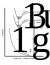
\includegraphics[width=0.7\textwidth]{images/Detector/RecombinationProcessFull.pdf}
    \caption[Full Cycle of the Ionisation/Excitation and Recombination Process]{This figure shows the full cycle of the ionisation/excitation and recombination process. On the $x$-axis we find the nuclear separation a designated argon atom changing its state and a fixed argon atom left at the ground state. The $y$-axis shows the energy of the designated argon atom. (1) indicates the excitation process of our designated atom, \ce{Ar -> \ch{Ar^*}}, after which the resulting exciton is dynamically trapped (2) and forms \ch{Ar2^*} with our fixed atom. (3) is the ionisation process, \ce{Ar -> \ch{Ar^+}} and (4) the rarely occurring direct recombination, \ce{\ch{Ar^+} + $e^-$ -> \ch{Ar^*}}, indicated by the dashed line. In (5) the designated argon ion is self-trapped and forms \ch{Ar2^+} with our fixed argon atom. (6) constitutes the recombination of the self-trapped ion to an \gls{excimer} argon \gls{excimer} \ce{\ch{Ar2^+} + $e^-$ -> \ch{Ar2^*}}. The wavy line denoted by (7), illustrates the scintillation process where the \gls{excimer} decays into its ground state, \ce{$^{1,3}\Sigma^+_{u}$ -> $^1\Sigma^+_{g}$}. Finally, the repulsive ground state $^1\Sigma^+_{g}$ relaxes again into two argon atoms, closing the cycle in (8). Above graph is an adaptation sourced from \cite{LArSelf-Trapping}.}
    \label{fig:FullRecombinationProcess}
\end{figure}

The two photon components emitted in the scintillation processes of equation \ref{eq:Scintillation} are not distinguishable in wavelength and thus the spectrum is characterised by a single peak with a maximum $\lambda_\text{sc} \approx \SI{128}{\nano\metre}$ \cite{LArScintillationSpectrum1,LArScintillationSpectrum2}. A graph of the scintillation spectrum of liquid argon is shown in figure \ref{fig:EmissionSpectrum}.
\begin{figure}[htbp]
    \centering
    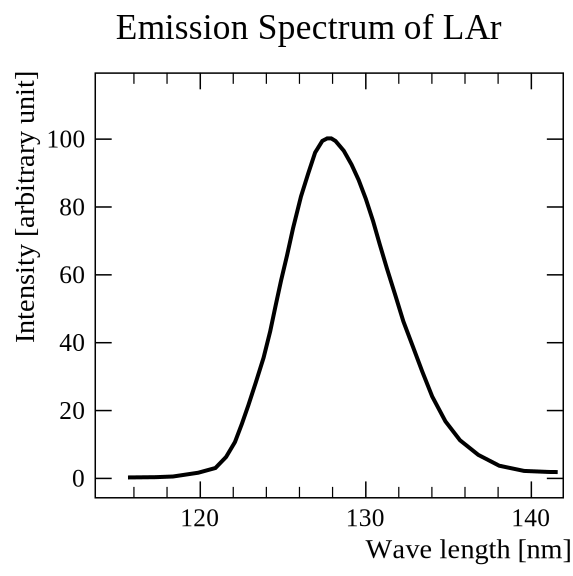
\includegraphics[width=0.7\textwidth]{images/Detector/EmissionSpectrum.pdf}
    \caption[Emission Spectrum of Liquid Argon]{This graph shows the emission (scintillation) spectrum of liquid argon at a temperature of \SI{87}{\kelvin}, redrawn from \cite{LArScintillationSpectrum2}. On the x-axis, the emission wave length is shown while the y-axis represents the intensity in arbitrary units. The spectrum's maximum is around \SI{128}{\nano\metre}.}
    \label{fig:EmissionSpectrum}
\end{figure}
Actually, the direct transition of the triplet state into the ground state \ce{^{3}\Sigma^+_u -> ^{1}\Sigma^+_g} is forbidden, but still occurs, owing to mixing between \ce{^{3}\Sigma^+_u} and \ce{^{1}\Pi_u} through spin-orbital coupling \cite{LArScintillationProcess1}. Thus the decay time of \ce{\ch{Ar2^*}(^{3}\Sigma^+_u)} is much longer, than the one of the \ce{\ch{Ar2^*}(^{1}\Sigma^+_u)} state. For this reason one distinguishes the fast component (\gls{singletexcimer}) with a lifetime of $\tau_\text{s} = \SI{7.0(10)}{\nano\second}$, and the slow component of the scintillation light (\gls{tripletexcimer}) with a lifetime of $\tau_\text{t} = \SI{1.6(1)}{\micro\second}$ \cite{LArScintillationTime}. The ratio of fast and slow component varies with the incident particle type and energy, \ie its linear stopping power; the higher the energy deposited by a particle, the higher the fraction of the fast component \cite{NobleGasDetectorsBetter}. The different scintillation component ratios for \SI{1}{\mega\electronvolt} electrons and \SI{5.4}{\mega\electronvolt} \textalpha-particles are visualised in figure \ref{fig:ScintillationFraction} below. 
\begin{figure}[htbp]
    \centering
    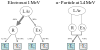
\includegraphics[width=0.8\textwidth]{images/Detector/ScintillationFraction.pdf}
    \caption[Luminosity Ratio of the Slow and Fast Components of Scintillation Light]{This figure shows the different ratios of the fast and slow components of scintillation light in \gls{lar} for \SI{1}{\mega\electronvolt} electrons and \SI{5.4}{\mega\electronvolt} \textalpha-particles. The letter \textbf{R} indicates the recombination origin of the emission, and \textbf{Ex} the exciton origin, respectively. This graph is sourced from \cite{NobleGasDetectorsBetter}.}
    \label{fig:ScintillationFraction}
\end{figure}
The formation of these \ch{Ar2^*} states is incidentally the reason for there being any measurable scintillation light. A decay photon of a simple excited state \ch{Ar^*} would be absorbed through \gls{selfabsorption} and re-emitted multiple times by the dense argon surrounding it (\ce{\ch{Ar^*} <=> Ar + $\gamma$}). Said process is called trapping of resonant radiation and renders the light useless for detection, especially in dense noble liquids. Since there are no naturally occurring ground state \glspl{excimer} \ce{Ar2($^1\Sigma^+_{g}$)} in \gls{lar}, the scintillation light exhibits no resonance to the ground state argon \ce{Ar} surrounding it and is not subject to \gls{selfabsorption}. In other words there is no reverse process to the scintillation light generation of equation \ref{eq:Scintillation}. Hence, \gls{lar} is transparent to its own scintillation light. After its genesis, the scintillation light traverses the \gls{lar} with the speed of light and is eventually either detected by the light readout system (see section \ref{sec:LightReadoutSystems}), or absorbed by other detector structures. Due to its excellent scintillation properties, \gls{lar} is even used in pure scintillation detectors like DEAP-3600 \cite{DEAPExperiment}. \gls{lartpc} experiments like MicroBooNE, however, mostly use the scintillation light as a trigger, \ie to determine the $t_0$ of particle interactions, and do not make use of all the additional information it provides. 

In order to quantify the scintillation light production a W-value, $W_\text{ph}$, is introduced, similar to $W_\text{i}$ in equation \ref{eq:W-ValueDefinition}. $W_\text{ph}$ has also a similar meaning, as it denotes the mean energy an incident particle charged particle, $X^{\pm}$, expends in order to produce a single scintillation photon. The mathematical definition of the W-value for scintillation light is given by
\begin{equation}\label{eq:W-ScintillationDefinition}
    W_\text{ph} \coloneqq k_{\text{i}} I_\text{LAr} + \frac{N_{\text{ex}}}{N}\bar{I}_{\text{ex}} + \bar{\epsilon}_{\text{se}}.
\end{equation}
Note that above equation presumes the production of scintillation light with no electric field applied. In the $W_\text{ph}$ definition we now use the ionisation potential $I_{\text{LAr}}$ and the average excitation potential $\bar{I}_{\text{ex}}$ instead of average expended energy of a particle $\bar{E}_{\text{i}}$ and $\bar{E}_{\text{ex}}$. Further, the form factor $k_{\text{i}}$ is introduced to account for multiply charged and excited charged states, and lastly $\bar{\epsilon}_{\text{se}}$ denotes the average kinetic energy of subexcitation electrons. The later can be understood as the inefficiency of the scintillation light genesis. There are, however, various values of $W_\text{ph}$ for different incident particles and their deposited energy. For heavy relativistic ions $W_\text{ph}$ was measured by T. Doke and K. Masuda \cite{LArWScint-Value1} in \gls{lar} as $W_\text{ph}(\text{max}) = \SI{19.5(10)}{\electronvolt}$. This value also constitutes the maximum yield and is therefore tagged with $\text{max}$. The same physicists also found different values for relativistic electrons close to \gls{mip} energy with $W_\text{ph}(\beta) = W_\text{ph}(\text{MIP}) = \SI{25.1(25)}{\electronvolt}$ and for \textalpha-particles with $W_\text{ph}(\alpha) = \SI{27.5(28)}{\electronvolt}$, respectively. This means that for those two particles the light yield is lower than for heavy relativistic ions. In case of the relativistic electrons the cause for the lower yield is, the low ionisation density along the particle track. This enables some valence electrons to break free from their parent-ions, even without an electric field applied. In other words the electron's thermal energy is higher than the Coulomb potential of the ions and they become so-called \textbf{escape electrons} \cite{LArScintillationEscapeElectron,LArWScint-Value2}. The reason for the lower emission yield of \textalpha-particles lies in the process of \textbf{bi-excitonic quenching}. Said process takes place before the \gls{dynamicaltrapping} of excited states and thus inhibits (quenches) the formation of \ch{Ar2^*} and with it the scintillation light emission. \textbf{Bi-excitonic quenching} is the process of two excited atoms \ch{Ar^*} exchanging the excitation energy while ionising one of them and relaxing the other to its ground state, \ie
\begin{equation}
    \ce{\ch{Ar^*} + \ch{Ar^*} -> Ar + Ar^+ + $e^-$}.
\end{equation}
The excess energy of this reaction is transformed to kinetic energy of the electron, which then becomes an \textbf{escape electron} as described above. This quenching can only occur if the density of excited states \ch{Ar^*} reaches a relatively high level, which is only achieved by incident particles with a high energy transfer to \gls{lar} \cite{LArScintillationQuenching}. Latter is certainly the case for \textalpha-particles, given their relatively high linear stopping power shown in figure \ref{fig:BetheBloch}.

There is also a measurable attenuation of scintillation light due to impurities in the detector medium. It is mainly caused by two impurities in \gls{lar}, \ce{N2} and \ce{O2}, through an additional quenching processes in the early stages of the scintillation light genesis. In the case of \ce{N2} said interference can occur even before the \gls{dynamicaltrapping}, \ie the production of \ch{Ar2^*} (see equation \ref{eq:ExcimerProduction}), can occur. During this quenching, the \ce{N2} molecule collides with the \ch{Ar^*} and the excitation is transmitted \cite{LArScintillationQuenchingN1}, \ie
\begin{equation}
    \ce{\ch{Ar^*} + N2 -> Ar + \ch{N2^*}}.
\end{equation}
Although the excited nitrogen molecule \ch{N2^*} would decay under emission of a photon, it would be in a different wave length and in a different lifetime compared to \ch{Ar2^*} and thus distort the scintillation signature. Above reaction is rather rare at low impurity levels of \si{\ppm} scale, since the \gls{dynamicaltrapping} occurs in a very short time period of \SI{6e-12}{\second}, as established earlier. The quenching takes much longer with $\sim \SI {8e-6}{\second}$ at \SI{1}{\ppm} \cite{LArScintillationQuenchingN2}. Thus the following reactions are dominating the impurity quenching effect for \ce{N2} and \ce{O2},
\begin{align} \label{eq:ScintillationQuenching}
    \ce{\ch{Ar2^*} + N2 -> 2Ar + N2 + \text{heat}}, \\
    \ce{\ch{Ar2^*} + O2 -> 2Ar + O2 + \text{heat}}. \nonumber
\end{align}
Unlike the aforementioned example, these processes are non-radiative, \ie the excitation energy is transformed fully into kinetic energy of the reaction products. As a result, the population of the photon precursors \ch{Ar2^*} is depleted before light emission \ie the emission is quenched \cite{LArScintillationQuenchingN2,LArScintillationQuenchingO2}. The effects of nitrogen and oxygen quenching have been studied extensively, and are found to reduce the scintillation yield by significant quantities at high impurity levels. A \ce{N2} impurity level of \SI{20}{\ppm} was found to reduce the emission intensity by $\sim \SI{60}{\percent}$ \cite{LArScintillationQuenchingN2}, while the same quenching is found at an \ce{O2} level of already \SI{10}{\ppm} \cite{LArScintillationQuenchingO2}. Both impurities show no effect of quenching below a \SI{0.1}{\ppm} concentration. Furthermore, the quenching seems to affect predominantly the slow component of the scintillation light, which means that the impurities predominantly interact with the \gls{tripletexcimer} \ce{\ch{Ar2^*}(^{3}\Sigma^+_u)}. This can be explained by the triplet's much longer lifetime, whereby the impurities have more time to collide with \gls{excimer}. Thus, the impurities have a higher chance of quenching the triplet than the singlet state. In a \gls{lartpc} experiment, \ce{O2} contamination levels are usually mitigated by the use of active copper filters, which are able to bind the oxygen due to its high \gls{electronegativity}. Hence, \ce{O2} contamination does not pose a problem with regards to scintillation light. \ce{N2} levels, on the other hand, are mostly not even measured and, because of the molecules low \gls{electronegativity}, can not be filtered as easily as \ce{O2}. It can be assumed that the \ce{N2} impurity levels would slowly increase in the detector with the passing of time, as a result of small leaks in the cryogenic system, and thus quench emission yields more and more. Thus it is paramount for large scale experiments with long running times to mitigate this problem with molecular sieves or hot metal getters made of titanium or barium. Impurities can also shorten the lifetime of the two \glspl{excimer} along with quenching. It is hypothesised, that soft collisions with impurities may induce an immediate decay \cite{LArScintillationTime}. This shortens the slow component's lifetime $\tau_\text{s}$ in particular, since, again, a longer lifetime increases the chance of a collision.

Recombination and scintillation are studied in much detail, still there are major unknowns for \gls{lartpc} applications; especially in the characteristics of scintillation and its W-value $W_\text{ph}$. Similar to $W_\text{i}$, $W_\text{ph}$ is used in a very liberal way by the neutrino physics community leading to several problems:
\begin{enumerate}
    \item $W_\text{ph}(\text{max}) = \SI{19.5(10)}{\electronvolt}$ is used for all particles, although we are mostly dealing with \glspl{mip} and thus $W_\text{ph}(\text{MIP}) = \SI{25.1(25)}{\electronvolt}$ would probably suit better.
    \item $W_\text{ph}$ has been measured using sources in a limited energy range of the order of \SI{1}{\mega\electronvolt}.
    \item So far $W_\text{ph}$ has not been determined for muons, pions, or protons at all.
    \item The effect of the \gls{lar} density, and thus pressure and temperature, on $W_\text{ph}$ are not measured at all.
\end{enumerate}
The measurements so far were obviously tuned for dark matter research purposes and it is time for the neutrino community to catch-up, even if our needs in regard of scintillation might not be pressing, since it is often only used as a trigger signal. I am certain, that there is a lot of use for a well understood scintillation signal and it could help to achieve more accurate particle identification in \glspl{lartpc}. Therefore a measurement of $W_\text{ph}$ as a function of linear stopping power would be of great value.
% TODO calculate photons per mm with W_ph(MIP)

\section{Charge Carrier Drift} \label{sec:ChargeDrift}
Hitherto we examined rather fast processes occurring in \gls{lar}: the formation of an ionisation track by a charged particle $\mathcal{O}(\SI{e-9}{\second})$, recombination $ < \mathcal{O}(\SI{e-9}{\second})$, \gls{selftrapping} $\mathcal{O}(\SI{e-12}{\second})$, and \gls{excimer} decay, \ie scintillation light genesis, up to $\mathcal{O}(\SI{e-6}{\second})$. Now we will examine the slowest process in a \gls{lartpc}, which is the charge drift. In MicroBooNE sized detectors we observe drift time scales of $\mathcal{O}(\SI{e-3}{\second})$ for \glspl{quasifreeelectron} and $\mathcal{O}(\SI{e3}{\second})$ for ions. \Glspl{quasifreeelectron}, $e^-$, and self-trapped argon ion dimers, \ch{Ar2^+}, which were not experiencing recombination, are then subject to charge carrier drift. In \gls{lar} these point like \glspl{quasifreeelectron} are able to move fast, while the rather large \ch{Ar2^+} ions show an impaired movement behaviour. In addition, these self-trapped dimers are not stable and the charge is able to transfer onto randomly colliding \ce{Ar} atoms which again will be self-trapped. This behaviour screens the charge of the ion, thus increasing its effective mass and further reduces its ability to move also known as \gls{mobility} \cite{NobleGasDetectors}. Note, that the drifting ion species was indeed identified as \ch{Ar2^+} in several measurements \cite{LArMobilityPressure,LArIonDrift1}.

Charge drift is the motion of charge carriers induced by an electric field $\vec{E}$. So in order to achieve a consistent drift, every \gls{tpc}'s field cage is designed in such a way that $\vec{E}$ is as uniform as possible. In case of negatively charged carriers, \eg $e^-$, said motion is vectored against the direction of $\vec{E}$ and thus towards the anode, while positively charged carriers, \eg \ch{Ar2^+}, move with the field vector towards the cathode. The relation between a charge carrier's drift velocity $v_e$ and the electric field strength $E \coloneqq \abs*{\vec{E}}$ is mathematically described as follows \cite{LArElectronDrift1}:
\begin{equation}\label{eq:DriftVelocity}
    v_e(\rho,E) = \mu(\rho,E) E.
\end{equation}
The proportionality function $\mu(\rho,E)$ is called \gls{mobility} and is typically expressed in units of $[\si{\centi\metre\squared\per\second\per\volt}]$ \cite{NobleGasDetectors}. It is a function of $E$ and the drift medium density $\rho$ and thus also dependent on the temperature $T$ \cite{LArMobilityTemperature} and the pressure $p$ \cite{LArMobilityPressure}. A special case of said \gls{mobility} is $\mu_0$ called \gls{zero-fieldmobility} and it is only suitable for small electric field strengths, \ie $\mu = \mu_0$ if $E \to 0$. At these limits it still depends on the medium's density but looses its $E$ dependency. Thus, the drift velocity in equation \ref{eq:DriftVelocity} becomes linear in $E$. In the case of \glspl{quasifreeelectron} in \gls{lar}, the aforementioned linearity and thereby $\mu_0$ are only applicable for $E \lesssim \SI{150}{\volt\per\centi\metre}$, \ie for a rather small range in electric field strength. For a drift electron in \gls{lar} at standard \gls{bp}, the \gls{zero-fieldmobility} is measured as \cite{LArElectronMobility}
\begin{equation} \label{eq:ConstMobility}
    \mu_{0,e} = \SI{516(27)}{\centi\metre\squared\per\second\per\volt}.
\end{equation}
Above \SI{150}{\volt\per\centi\metre}, the electron drift velocity $v_e$ nears and later exceeds the velocity of sound waves (phonons) in \gls{lar} at $c_\text{s} = \SI{842.9(84)}{\metre\per\second}$ \cite{NistChemistryWebBook}. As a consequence the resistance for the drifting electrons in the liquid increases whereby the electron \gls{mobility} $\mu_e$ decreases. Thus the function of $v_e(E)$ flattens with increasing field strength $E$. Heretofore, nobody developed a reliable model of the aforementioned increase in resistance and thus it is best described by an empirical equation \cite{LArElectronDriftFunction}:
\begin{equation}
    v_e(T,E) = \left( 1 + P_1 \left( T - T_0 \right) \right) \left( P_3 E \ln{\left(1+\frac{P_4}{E}\right)} + P_5E^{P_6} \right) + P_2\left( T - T_0 \right).
\end{equation}
The parameters $P_i$ are usually fitted to data points in the region of interest of the corresponding experiment, whereby $T_0$ is set to be the temperature at which the data points were collected. This leads to stitched together functions for $v_e(E)$ when regarding greater intervals in $E$, as is shown in figure \ref{fig:DriftVelocity}. It depicts $v_e(E)$ between \num{0} and \SI{10}{\kilo\volt} at the \gls{bp} temperature $T = \SI{87.303}{\kelvin}$.
\begin{figure}[htbp]
\centering
\includegraphics[width=0.9\textwidth]{images/Detector/DriftVelocityElectron.pdf}     
\caption[Electron Drift Velocity as a Function of Electric Field]{This image depicts the electron drift velocity $v_e$ as a function of electric field strength $E$ from \SIrange{0}{10}{\kilo\volt} at a temperature of $T = \SI{87.303}{\kelvin}$ (\gls{bp} at \SI{1}{\bar}). In the small graph a magnified view of the same drift velocity between \SI{0}{\kilo\volt} and \SI{1}{\kilo\volt} is shown. The function used to draw this graph has three parts. First, from \SIrange{0}{0.15}{\kilo\volt}, the linear function \ref{eq:DriftVelocity} and $\mu_{0,e}$ of equation \ref{eq:ConstMobility} is used. Second, in the range from \SIrange{0.15}{0.7}{\kilo\volt}, an empirical function \cite{LArElectronDriftFunction} with parameters obtained from \cite{LArElectronDrift3} is employed. Third, above \SI{0.7}{\kilo\volt}, the same empirical function is applied with different parametrisation \cite{LArElectronDrift2}. The black vertical line shows the velocity of sound $c_s$.}
\label{fig:DriftVelocity}
\end{figure}
% TODO Draw line where microboone is at!

While drifting, all charge carrier clouds are subject to diffusion, rooted in their Brownian motion. In three dimensions and without an electric field said diffusion is mathematically described by Einstein's abundance distribution \cite{BrownianMotion}
\begin{equation} \label{eq:DiffusionEquationOrigin}
    n(t,\vec{x}) = \frac{N_0}{\left(4 \pi D t \right)^{\frac{3}{2}}} \, e^{-\frac{\vec{x}^2}{4Dt}},
\end{equation} 
with $n(t,\vec{x})$ denoting the number density of the charge carriers at time $t$ and location $\vec{x}$, $N_0$ the total number of charge carriers in the cloud, and $D$ the diffusion coefficient. Above diffusion function will be infinitesimally thin in space at $t=\SI{0}{\second}$ and will spread more with increasing $t$, while its integral remains constant. Therefore, diffusion is observed in a \gls{lartpc} as a spacial spread of the charge signal, widening with drift time. To characterise said spacial spread, the standard deviation $\sigma$ of above distribution is used which is given by \cite{BrownianMotion}
\begin{equation} \label{eq:DiffusionWidthOrigin}
    \sigma = \sqrt{2Dt}.
\end{equation}
The diffusion coefficient $D$ itself is dependent on the energy distribution of the charge carriers. In case of \glspl{quasifreeelectron} in absence of a drift electric field, $D$ is given by the Nernst-Townsent relation for charged particles \cite{LArDiffusionTheory1}
\begin{equation}
    \frac{D}{\mu_0} = \frac{kT}{q},
\end{equation}
with $k$ being the Boltzmann's constant, $T$ the temperature, and $q$ the charge of the particle ($q=e$ in case of $e^-$). The $kT$ part of the equation shows that, in this case, $D$ depends purely on the thermal energy of the charge carrier. It is also interesting to see, how the diffusion coefficient is directly related to the \gls{zero-fieldmobility} $\mu_0$. This makes perfect sense, since it implies that the charge carrier faces the same resistance for Brownian motion and the drift in a weak electric field. In case of electrons, we are able to calculate the diffusion coefficient at standard \gls{bp} and without any drift field as $D = \SI{3.9}{\centi\metre\squared\per\second}$. Applying an electric field also increases the energy of the charge carrier which in turn influences the diffusion coefficient $D$. For electrons, this change is significant and $D$ takes the form \cite{LArDiffusionTheory1,LArDiffusionTheory2}
\begin{equation}
    \frac{D}{\mu} = F \frac{ \bar{\varepsilon}}{e},
\end{equation}
where $\mu$ is now used instead of $\mu_0$ and variable $\bar{\varepsilon}$ denotes the mean electron energy. $F$ is a constant depending on the electron momentum distribution. In case of a Maxwell distribution of electron momenta $F=2/3$ \cite{LArDiffusionTheory1}. The kinetic theories of electrons in \gls{lar}, \ie the derivation of $F$ and $\bar{\varepsilon}$, are by themselves a vast topic and are thus not discussed here. However, I would like to reference the most significant works on this topic by M.H. Cohen and J. Lekner \cite{LArElectronKinematics1,LArElectronKinematics2} as well as V.M. Atrazhev and I.V. Timoshkin \cite{LArDiffusionAnisotropy}. In case of large enough $\bar{\varepsilon}$ the electrons are considered ``hot'' and diffusion looses its isotropy, \ie it becomes directional. It is thus split into two components: the longitudinal component in the $x$-coordinate, parallel to the electric field, governed by $\bar{\varepsilon}_\text{L}$ and its derived diffusion coefficient $D_\text{L}$, and the transverse component in the $y$-$z$-plane perpendicular to the field driven by $\bar{\varepsilon}_\text{T}$ and $D_\text{T}$ \cite{LArDiffusionTheory1,LArDiffusionAnisotropy}. Therefore, let us rewrite the diffusion equation \ref{eq:DiffusionEquationOrigin} as \cite{LArDiffusionTheory1}
\begin{equation} \label{eq:DiffusionEquation}
    n(t,\vec{x}) = \frac{N_0}{4 \pi D_\text{T} t \sqrt{4 \pi D_\text{L} t}} \,e^{-\frac{(x - v_et)^2}{4D_\text{L}t}} e^{-\frac{y^2+z^2}{4D_\text{T}t}},
\end{equation}
where the charge position in the $x$-coordinate now also includes the drift with velocity $v_e$. Above described anisotropy can be subsequently observed in the difference of spacial spread of the charge cloud from equation \ref{eq:DiffusionWidthOrigin} becomes
\begin{equation} \label{eq:DiffusionWidth}
    \sigma_\text{L,T} = \sqrt{\frac{2xD_\text{L,T}}{\mu E}},
\end{equation}
while also converting time $t$ by employing the drift distance $x$, the \gls{mobility} $\mu$, and the electric field strength $E$. Measurements of electron diffusion in \gls{lar} are sparse and often contradicting, see table \ref{tab:Diffusion}.
\begin{table}[hbtp]
    \centering
    \caption[List of Electron Measured Diffusion Coefficients $D_\text{L,T}$ in LAr]{List of measured electron diffusion coefficients $D_\text{L,T}$ in \gls{lar}. There are only a few known measurements of $D_\text{L}$ and some of them seem to differ strongly, although they were measured at similar electric field strengths $E$. For $D_\text{T}$ there is only one known measurement.}
    \begin{tabu} to 0.9\textwidth{cccc} \toprule
        \rowfont[c]{\bf}Measured Coefficient & $\mathbf{E}\ [\si{\volt\per\centi\metre}]$ & $\mathbf{D_{L,T}}\ [\si{\centi\metre\squared\per\second}]$ & Source \\ \midrule
        \multirow{7}{*}{$D_\text{L}$} & \num{0}   & \num{4.5} & \multirow{7}{*}{\cite{LArElectronDiffusionL1}} \\
                               & \num{300} & \num{9.0} & \\
                               & \num{1000} & \num{13} & \\
                               & \num{3000} & \num{18} & \\
                               & \num{1e4} & \num{24} & \\
                               & \num{3e4} & \num{33} & \\
                               & \num{1e5} & \num{34} & \\ \midrule
        \multirow{3}{*}{$D_\text{L}$} & \num{2000} & $\sim \num{3}$ & \multirow{3}{*}{\cite{LArDiffusionTheory2}} \\
                               & $\vdots$ &  $\vdots$ & \\
                               & \num{1e4} & $\sim \num{16}$ & \\ \midrule
        $D_\text{L}$           & \num{100} & \num{4.8(2)} & \cite{LArElectronDiffusionL2} \\ \midrule
        $D_\text{L}$           & \num{120} & \num{5.3(5)} & \cite{Argontube1} \\ \midrule
        $D_\text{T}$           & \num{2700} & \num{15} & \cite{LArElectronDiffusionT} \\ \bottomrule          
    \end{tabu}
    \label{tab:Diffusion}
\end{table}
Considering the most recent theory \cite{LArDiffusionAnisotropy} the longitudinal diffusion component over the full drift length in MicroBooNE is given as $\sigma_\text{L,max} = \SI{1.3}{\milli\metre}$ and the transverse component is expected to be $\sigma_\text{T,max} = \SI{2.0}{\milli\metre}$. The latter can not be observed in MicroBooNE because of its $y$-$z$-resolution of only \SI{3}{\milli\metre}. Hence, diffusion does not interfere with an accurate charge measurement. The effect of diffusion in the MicroBooNE detector over time is shown in figure \ref{fig:Diffusion}.
\begin{figure}[htbp]
\centering
\includegraphics[width=0.9\textwidth]{images/Detector/Diffusion.pdf}     
\caption[Longitudinal Component of the Electron Diffusion Function for Various Drift Times]{Above illustration shows the longitudinal component of the electron diffusion function $n(t,z)/N_0$ (see equation \ref{eq:DiffusionEquation})  with $z = z\prime + v_e*t$ for the drift times \SIlist[list-units = single]{0.05;0.50;2.25}{\milli\second}. The coordinate shift centres all distributions around \SI{0}{\centi\metre} and thus allows for a direct comparison of the $e^-$ distributions. All distributions are calculated using MicroBooNE's operational electric field strength of \SI{273.4}{\volt\per\centi\metre} and the corresponding $\bar{\varepsilon}_{L}$ sourced from \cite{LArDiffusionAnisotropy}. In addition the drift time of \SI{2.25}{\milli\second} corresponds to a full drift from cathode to anode in the MicroBooNE detector during regular operations.}
\label{fig:Diffusion}
\end{figure}

While the charge carriers drift in \gls{lar} they not only undergo diffusion but also collide with impurities. Depending on their \gls{electronegativity}, these impurities are able to capture the charge. This attachment process is predominantly prevalent with \glspl{quasifreeelectron} and can be described as \cite{LArPurity1}
\begin{equation} \label{eq:ImpuitiesGeneral}
    \ce{e^- + S ->[$k_\text{S}$] S^-},
\end{equation}
where \ce{S} is the electronegative impurity molecule and $k_\text{S}$ denotes the rate constant of this process in units of $[\si{\per\mole\per\second}]$. Above process inevitably leads to a reduction of the charge signal in a \gls{tpc}. If the impurities are homogeneously distributed throughout the detector's active volume, said reduction can be described as an exponential attenuation \cite{LArPurity2}
\begin{equation} \label{eq:ChargeAttinuation}
    Q(t) = Q_0 e^{-\frac{t}{\tau}}.
\end{equation}
Here, $Q(t)$ is the amount of \glspl{quasifreeelectron} left after a drift time $t$, $Q_0$ the number of \glspl{quasifreeelectron} right after recombination, and $\tau$ the \textbf{charge lifetime}. The latter is connected to the abovementioned rate constant $k_\text{S}$ \cite{LArPurity3}
\begin{equation} \label{eq:ChargeLifetime}
    \tau = \frac{1}{k_\text{S}n_\text{S}},
\end{equation}
where $n_\text{S}$ denotes the amount of substance \ce{S} in $[\si{\mole}]$. For an accurate charge measurement and reconstruction in a \gls{lartpc} the fraction $Q(t)/Q_0$ needs to be determined, in order to compensate the impurity induced attenuation and reconstruct the ionisation signal. This can be achieved by measuring $Q(t)$ of a constant ionisation source like a \gls{uv}-laser over a variable $t$ \cite{Argontube0} or by determining $Q(t_\text{d})/Q_0$ over a fixed drift time $t_\text{d}$ employing the photoelectric effect \cite{PhotoelectricEffect} of a \gls{uv} flash lamp on the cathode, like in a purity monitor \cite{LArPurityMonitor,LArPurifying}. There are several impurities identified to capture drifting \glspl{quasifreeelectron}, these are: sulphur hexafluoride \ce{SF6}, carbon dioxide \ce{CO2}, nitrous oxide \ce{N2O}, water \ce{H2O}, and oxygen \ce{O2}. Only the latter two, \ce{H2O} and \ce{O2}, are relevant in a \gls{lartpc} as they are the only ones appearing in our atmosphere in considerable amounts. The trapping of \glspl{quasifreeelectron} $e^-$ by most of these impurities, described in equation \ref{eq:ImpuitiesGeneral}, actually occurs in two stages. First, the electron is captured whereby an excited charge state of the impurity is produced. Then, said excited impurity is then relaxed through a collision with a third body, most likely an argon atom \ce{Ar}. The following example shows aforementioned two stage trapping process for an oxygen impurity in \gls{lar} \cite{LArPurity1}:
\begin{align}
    \ce{e^- + O2 &-> \ch{O2^{-*}}} \nonumber \\
    \ce{\ch{O2^{-*}} + Ar &-> \ch{O2^- + Ar^*}}.
\end{align}
All the above impurities exhibit different $k_\text{S}$, which again are $E$ dependent. For MicroBooNE's operating electric field $k_{\ce{O2}} \approx \SI{1e11}{\per\mole\per\second}$, $k_{\ce{H2O}} \approx \SI{8e11}{\per\mole\per\second}$, and the impurity capturing the electrons the strongest $k_{\ce{SF6}} \approx \SI{1.5e14}{\per\mole\per\second}$ \cite{LArPurity1}. In the field of \glspl{lartpc}, oxygen holds a special role in impurity measurements. It serves as a gauge for all electron trapping impurities and thus the term \textbf{oxygen equivalent impurity level} is often used. By doing this, all impurities are assigned the rate constant $k_{\ce{O2}}$ and thus a \ce{H2O} molecule for example would be counted as eight \ce{O2} molecules. In \gls{lar} the oxygen equivalent impurity level, $n_{\ce{O2}}$, is mostly expressed in units of parts per billion $[\si{\ppb}]$ and can be derived adapting equation \ref{eq:ChargeLifetime} as \cite{LArPurity2,LArPurity3}
\begin{equation}
    n_{\ce{O2}} [\si{\ppb}] = \frac{\num{300}}{\tau [\si{\micro\second}]}
\end{equation}
Typical achieved charge lifetimes $\tau$ are of the order of several milliseconds, wherefore oxygen equivalent impurity level $n_{\ce{O2}}$ are usually found in the range from \SIrange{0.3}{0.03}{\ppb}. A stable impurity level can only be achieved by persistent purification. This is attributed to small leaks in the cryo-system and outgassing from built-in components. Said purification is achieved by sintered copper filters and molecular sieves, through which \gls{lar} is circulated by powerful pumps.

% TODO refrase  first sentence
In the case of positively charged argon dimers, \ch{Ar2^+}, the drift velocity is in accordance with the linear function \ref{eq:DriftVelocity}. This time the direction of motion is the same as $\vec{E}$, \ie the opposite direction of the \gls{quasifreeelectron} drift. Since the ion's \gls{mobility} stays constant over a wide range of electric field strength (at least up to \SI{10}{\kilo\volt}) \cite{LArIonDrift2}, there is no need for further complicated empirical equations to describe their movement. The reason for this stability lies in the very slow drift velocity of ions, $v_\text{i}$, which is far below the phonon velocity $c_s$. In fact the \gls{zero-fieldmobility} of argon ions $\mu_{0,\text{i}}$ is six orders of magnitude smaller than $\mu_{0,e}$ and at standard \gls{bp} takes the value of \cite{LArMobilityTemperature}
\begin{equation}
    \mu_{0,\text{i}} = \SI{1.5e-3}{\centi\metre\squared\per\volt\per\second}.
\end{equation}
Using equation \ref{eq:DriftVelocity}, this results in $v_\text{i}$ of the order of \SI{1}{\centi\metre\per\second} in most \gls{lartpc} experiments, which is of the same magnitude as \gls{lar}-flow speeds. At the operational field strength of MicroBooNE, for instance, we find an ion drift velocity of only $v_\text{i} = \SI{0.41}{\centi\metre\per\second}$, which corresponds to a full drift time in excess of roughly \SI{10}{\minute}. Since \ch{Ar2^+} ions dwell for tens of minutes in a \gls{lartpc} the size of MicroBooNE, they are subject to diffusion on a large time scale. Therefore, a large amount of ions is used to measure their mobility. But large amounts of drifting \ch{Ar2^+} themselves contribute significantly to the flow of \gls{lar}, thereby distorting the measurement. Thus, measurements of $\mu_{0,\text{i}}$ show great variations, from \SIrange{0.2e-3}{3.2e-3}{\centi\metre\squared\per\volt\per\second} \cite{LArMobilityPressure,LArIonDrift1,LArMobilityTemperature,LArIonDrift2}. In this work I chose the value that is most applied in the field. Note, that the same value of $\mu_{0,\text{i}}$ is also valid for the impurity ions, like \ch{O2^-} introduced above \cite{LArIonDrift2}. Their movement, however, is directed towards the anode instead of the cathode. Furthermore, I would hypothesise that the drifting argon ions, \ch{Ar2^+}, themselves act as impurities and thus contribute to the \gls{quasifreeelectron} trapping. Since their distribution is not homogeneous throughout the active volume, we have to assume their attenuation function to be more complicated than the one for \glspl{quasifreeelectron} of equation \ref{eq:ChargeAttinuation}. Moreover, the slow drift of the \ch{Ar2^+} ions also contributes to a distortion of the drift electric field of surface detectors. This effect is discussed in more detail in section \ref{sec:SpaceCharge}.

\section{Charge Readout} \label{sec:ChargeReadout}
Arriving at the anode, the clouds of drift electrons are eventually captured by the anode material and can thus be converted to electrical signals. This charge readout process should provide an exact position of the charge on the anode plane, \ie the $y$-$z$-plane. A simple solution for this problem appears to be an array of pixels, which are read out individually. However, this solution scales with $y \cdot z$ and thus generates many readout channels, while a readout channel constitutes the most expensive commodity in every particle detector. Thus, most large scale \glspl{tpc} still use wire plane readouts. Said readouts consist of at least two parallel planes. Within one plane all wires are parallel, but every plane exhibits a different wire angle to one another, \eg see MicroBooNE setup in figure \ref{fig:WirePlaneSetup}. This also provides positional information in $y$ and $z$, although this choice complicates signal reconstruction and introduces some ambiguity when electron clouds arrive at two different spots on the plane at the exact same time. The big advantage of wire plane charge readouts is undoubtedly the reduced scaling of the number of readout channels, from $y \cdot z$ to $y + z$, compared to a pixel array and thus resulting in reduced cost.

Using wire planes without taking additional measures, would result in the \gls{quasifreeelectron} clouds being collected by the first wire plane they encounter, while any plane behind would be shielded completely. In order to achieve the $y$-$z$ position measurement it is paramount to make said first plane transparent to the drift electrons. This is achieved by applying a bias voltage to the wire planes and thus inducing an electric field $\vec{E}_\text{b}$ between them. According to \cite{TPCWireSpacing} transparency of a wire plane is given when
\begin{equation} \label{eq:WireTransparency}
    \frac{E_{\text{b}}}{E_{\text{f}}} > \frac{1+\rho}{1-\rho}, \qquad \text{with} \quad \rho = \frac{2\pi r}{d}. % For microboone the right side rho = pi/10 -> right side = 1.915
\end{equation}
Here the wire plane's back side field strength $E_{\text{b}}\coloneqq \abs*{\vec{E}_\text{b}}$ and the front side field strength $E_{\text{f}}\coloneqq \abs*{\vec{E}_\text{f}}$ need to fulfil above condition. Furthermore, $r$ denotes the wire radius (typically of the order of \SI{100}{\micro\metre}) and $d$ the inter-wire spacing within the plane (typically of the order of \SI{1}{\milli\metre}). In the special case of the first wire plane, $E_{\text{f}}$ equates to the drift electric field strength $E$. The effect of said readout plane transparency on drifting \glspl{quasifreeelectron} is presented in figure \ref{fig:WireTransparency}.
\begin{figure}[htbp]
    \centering
    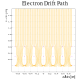
\includegraphics[width=0.6\textwidth]{images/Detector/WireTransparency.pdf}     
    \caption[Electron Drift Paths at the Readout Wire Planes]{The figure presented here depicts a \gls{2d} top view of simulated electron drift paths at the readout wire planes of the MicroBooNE \gls{tpc} \cite{LArTPCReadoutWires}. Shown in purple are the wire cross sections and the drift paths in orange. There are three wire planes: two induction planes on top and at the bottom one collection plane. As can be seen, the electrons circumvent the two induction planes and are collected by the collection plane.}
    \label{fig:WireTransparency}
\end{figure}
Using MicroBooNE's design specifications as an example, the wire plane transparency relation in equation \ref{eq:WireTransparency} is solved to $E_{\text{b}}/E_{\text{f}} > \num{1.92}$. This means that the electric field strength in the back of the induction plane needs to be at least \num{1.92} times larger than the field in the front.

If above transparency relation is satisfied, an approaching electron cloud starts to induce an increasing mirror charge and thus a current in the wires of the first plane. While passing the plane, the mirror charge is reduced and therefore the current reversed. This induction process leads to a bipolar current signal in the transparent plane, hence giving such plane its widely used designation: \gls{InductionPlane}. In order to reduce ambiguities during the reconstruction process, many large detectors like MicroBooNE, make use of two \glspl{InductionPlane}. An example Theoretically there is no limit to the number of induction planes, as long as the condition of equation \ref{eq:WireTransparency} is met. The signal shape of a two induction plane setup is shown in figures \ref{fig:U-PlaneSignal} and \ref{fig:V-PlaneSignal}. At the last plane the a high positive bias voltage is applied which leads to converging field lines onto the single wires (see figure \ref{fig:WireTransparency}). This guides the drift electrons to the wire where they are collected by the wire material. Therefore all experiments use gold coated wires in order to increase collection efficiency. The collected charge leads to a unipolar signal caused by the current of the captured drift electron flowing towards the bias voltage supply. Such collection signals are depicted in figure \ref{fig:Y-PlaneSignal}. Due to the charge collecting nature of the last plane it is called \gls{CollectionPlane}. The \gls{CollectionPlane} signal is the strongest and clearest signal type of a wire plane charge readout system, \ie highest signal-to-noise ratio. Therefore it is considered as the primary signal for event reconstruction and calorimetry. Most shown \gls{2d} event displays in the \gls{lartpc} field are collection plane signals. All charge signals first need to be amplified since they are too weak to process directly, \eg the collected charge of a \gls{CollectionPlane} wire is typically of the order of \SI{1}{\femto\coulomb} \cite{NobleGasDetectors}. The closer this amplification is performed to the readout wire, the better the recorded signal quality, as the noise level increases with conductor length. Nowadays it is standard to use cold amplifiers which are immersed in \gls{lar} and can be mounted directly at the end of the charge readout wire.

In my opinion, the future of \gls{lartpc} charge readout systems are pixelated solutions. First demonstrations of this technology were recently performed by the liquid argon group at \gls{lhep} at the University of Bern \cite{LArTPCReadoutPixels}. Then, apart from difficulties with event reconstruction, wire plane readouts exhibit relatively high noise levels compared to pixels. The main contributor in this regard are the wires themselves which act as perfect antennas for \gls{em} background. Another drawback is introduced by the bias voltage in order to achieve wire plane transparency. For this the signal path needs to be decoupled from the wire by a capacitor, which further worsens the noise situation. There are mechanical challenges too, since the wires must not touch each other, especially the ones from different planes because they would short the bias voltage supply. Thus engineers need to conceive elaborate tensioning systems and work with tight tolerances while producing the wire planes. All these challenges could be avoided by simply using a single pixel array which only works as a \gls{CollectionPlane}. With the dawn of new technologies like cold amplifiers and modern readout electronics becoming lower priced, the pixel readout plane will certainly be the charge readout of choice of future \glspl{lartpc}. This will also bring a direly needed boost in reconstruction accuracy.
\begin{figure}[htbp]
    \centering
    \subfloat[U-Plane Signal][U-plane induction signal]
    {
        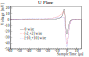
\includegraphics[width=0.5\textwidth]{images/Detector/WireSignalUPlane.pdf}
        \label{fig:U-PlaneSignal}
    } %\qquad
    \subfloat[V-Plane Signal][V-plane induction signal]
    {
        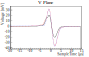
\includegraphics[width=0.5\textwidth]{images/Detector/WireSignalVPlane.pdf}
        \label{fig:V-PlaneSignal}
    }
    \\
    \subfloat[Y-Plane Signal][Y-plane collection signal]
    {
        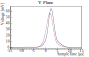
\includegraphics[width=0.5\textwidth]{images/Detector/WireSignalYPlane.pdf}
        \label{fig:Y-PlaneSignal}
    }
    \caption[Typical Wire Signal Wave Forms in a LArTPC]{This figure shows typical wire signal wave forms of a \gls{lartpc}. The wave forms presented above arise from the same MicroBooNE electron path simulation \cite{LArTPCReadoutWires} as introduced in figure \ref{fig:WireTransparency}. Here, the U-plane \subref{fig:U-PlaneSignal} denotes the first, and the V-plane \subref{fig:V-PlaneSignal} the second induction plane, while the Y-Plane \subref{fig:Y-PlaneSignal} is the collection plane. The black line designated ``\num{0} wire'' depicts the signal for charge drifting within one half pitch distance of a central wire. The coloured lines labelled by ``$[-N,+N]$ wire'' show the wave form on a central wire of longer charge tracks with a length of $N$ wire pitches on each side of the central wire. All tracks are parallel to the readout planes as well as horizontal to the earths surface.}
    \label{fig:WireSignals}
\end{figure}

%--------------------------------------------------------------------------------------------------------------------------
% \section{Adverse Effects of the Slow Drift}
\section{Light Readout Systems} \label{sec:LightReadoutSystems}
The goal of a light readout system is to convert in \gls{lar} produced scintillation light into an electric signal which provides intensity and time information. Therefore scintillation photons first need to be converted into electrons by the photoelectric effect. These electrons then need to be multiplied in a controlled manner and thereafter captured in order to induce a voltage. Finally, said voltage is amplified and digitised. The photon conversion and electron multiplication is achieved using \acrfullpl{pmt} or \glspl{sipm}.

A \gls{pmt} consists of a series of dynodes in vacuum tube made of glass. On the tube's top, one finds the photocathode which is usually just a glass surface metallised from the inside. On its bottom a \gls{pmt} features several electric contacts for the voltage supply of the dynodes as well as the signal readout. The photocathode is supplied by a bias voltage, usually between \SIrange{-0.5}{-2.5}{\kilo\volt}. A voltage divider then steps down the voltage for each dynode until the signal is read out at the ground dynode. \Glspl{pmt} can also be operated by connecting the cathode to ground and step up a positive voltage on the dynodes. In said case, a \gls{pmt} is operated in reverse bias mode. Whichever operation mode is chosen, the working principle stays the same: First a photon hits the photocathode and produces a \gls{pe} through the photoelectric effect. Accelerated by the electric field between the cathode and the first dynode, the electron, when hitting the dynode, produces secondary emission, \ie the impact of one high energy electron leads to the emission multiple electrons with lower energies. These secondary electrons are now again accelerated between the first and second dynode each again inducing secondary emission at the latter. This multiplication repeats itself after every dynode gap and results in electron gains of up to \num{e9}. The signal is prompt with rise times of about \SI{2}{\nano\second} and the event frequency can reach a couple of \SI{100}{\mega\hertz}. The concept of the \gls{pmt} was developed by H. Iams and B. Salzberg \cite{PMTFirst}.

The \gls{sipm} is a silicon chip with multiple independent pixels. Each pixel contains a p-n junction which is operated in Geiger-mode \cite{SiPMFirst}, \ie the junction is operated above its breakdown voltage. A breakdown in silicon is defined as electrons and holes gaining enough energy to create new electron hole pairs leading to an avalanche. If a photon now hits a pixel cell the breakdown is triggered within it, leading to gains up to \num{e6} \cite{SiPMReview}. The breakdown is quenched by high-ohmic resistors between the chip and the power supply, temporarily reducing the bias voltage across the p-n junction. Since the breakdown in a single cell always has the same characteristics independent of the amount of photons triggering it, the light intensity has to be measured by the amount of pixels producing a signal. Furthermore, the pixels are not read out individually, but the whole chip produces a signal according to the sum of all pixel signals. The operation in Geiger-mode also leads to spontaneous breakdowns constituting the so-called dark rate of a \gls{sipm} chip given by roughly $\SI{1}{\mega\hertz\per\milli\metre\squared}$ \cite{SiPMReview}. This dark rate can be significantly reduced by requiring a signal from multiple pixels, rather than from a single one.

As established before, scintillation light is emitted at \SI{128}{\nano\metre} wavelength. This poses a problem for a \gls{pmt}, because its photocathode is inside of the \gls{pmt}'s glass surface and glass is an excellent \gls{uv} light absorber. Thus wavelength shifting materials are used in \gls{lar} detectors in order to convert the \SI{128}{\nano\metre} \gls{uv} light into the visible range of the spectrum. The wavelength shifter most used in \glspl{lartpc} is \gls{tpb} \cite{TPB1,TPB2} an organic fluorescent substance able to convert \gls{uv} into visible light within picoseconds \cite{TPBTiming}. The emission spectrum of \gls{tpb} ranges from \SIrange{400}{525}{\nano\metre} (blue to green light) with a main peak at \SI{425(20)}{\nano\metre} \cite{TPBSpectrum}. \Gls{tpb} coatings are either applied directly to the glass surface of the \gls{pmt} or to a transparent (acrylic) shield in front of it. A major issue with \gls{tpb} is attributed to its degradation into benzophenone under \gls{uv} light exposure \cite{TPBDegradation}. Even worse, benzophenone is an commercially produced \gls{uv} blocker. Since benzophenone features an additional oxygen atom in its chemical structure compared to \gls{tpb}, said degradation only applies in oxygen rich environments. So, it can be assumed that principally the degradation of \gls{tpb} in ultra pure \gls{lar} should be of little relevance. However, most recent studies showed that \gls{tpb} emanates from the coatings into \gls{lar}, which could lead to a degradation of the light signal \cite{TPBDissolving}. Therefore, the community tries to find better solution than the \gls{tpb} - \gls{pmt} combination.

\glspl{sipm}, on the other hand, technically do not need a wavelength shifter, since they are not covered by an \gls{uv}-absorbent material. Short wavelengths are even advantageous as they also feature shorter absorption-lengths in silicon \cite{SiPMMasterBaeschu}. The disadvantage for a direct use is their size with only several square millimetre of active area. Still, \gls{sipm} based light readout systems are considered the future in the \gls{lartpc} community, since they provide better light intensity resolution and lower cost. In modern detectors a transparent polymer plate coated with dichroic reflectors and wavelength shifting materials are used as light traps in order to guide the light to an array of \glspl{sipm} \cite{SiPMLArTPC}. Although still not reaching the photon detection efficiency of a \gls{pmt}, such a light detection system is easily scalable and can thus partially compensate its deficiency by a larger area. MicroBooNE opted for the classical \gls{tpb}, \gls{pmt} approach, as the \gls{sipm} technology had not been tested in \gls{lar} at the date of the experiments conception.
% TODO Put this below recombination and scintillation chapter?
% TODO Maybe produce drawing of PMT and SiPM side by side?

\section{Electric Field Generation} \label{sec:LArElectricField}
In order to generate a uniform electric field in a \gls{tpc}, the supply of \gls{hv} to the cathode is essential and still poses a major limitation to \gls{tpc} sizes today. There are two methods employed to supply \gls{hv} to a \gls{lartpc}. The most common one provides the voltage directly from a \gls{dc} power supply to the cathode using a feedthrough to enter the cryostat. Resistors, typically of the order of \SI{100}{\mega\ohm}, between the field cage rings provide a regular step down of the voltage. Every resistor has the same resistance $R$ forming a so-called voltage divider circuit. This resistor chain is connected to ground at the anode. The described assembly provides a uniform electric field and is illustrated in figure \ref{fig:VoltageDivider}. Another, more exotic method is the \gls{hv} generation inside the cryostat employing a Cockcroft-Walton multiplier circuit fed by a lower voltage \gls{ac} power supply, typically several kilo volts. The Cockcroft-Walton circuit uses two chains of capacitors with a constant capacitance $C$ and one interlinked chain of diodes to pump electrons up the diode stages thus continuously multiplying the peak-to-peak input voltage by the stage number. Theoretically every stage can be connected to a field cage ring to achieve a regular voltage increase, see figure \ref{fig:CockcroftWalton}.
\begin{figure}[htbp]
    \centering
    \subfloat[Voltage Divider][Voltage divider circuit with \gls{dc} voltage supply]
    {
        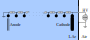
\includegraphics[width=0.7\textwidth]{images/Detector/TPCVoltageSupplyDC.pdf}
        \label{fig:VoltageDivider}
    }
    \\
    \subfloat[Cockcroft-Walton][Cockcroft-Walton multiplier circuit with \gls{ac} voltage supply]
    {
        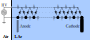
\includegraphics[width=0.7\textwidth]{images/Detector/TPCVoltageSupplyAC.pdf}
        \label{fig:CockcroftWalton}
    }
    \caption[TPC Field Cage Voltage Supply Methods]{Above figures show the two voltage supply methods for the field cage of a \gls{lartpc}. The field cage rings are depicted as filled black circles. In \subref{fig:VoltageDivider} the classical voltage divider is illustrated, with a resistor chain, connecting the field cage. In \subref{fig:CockcroftWalton} the complex circuit of the Cockcroft-Walton multiplier is shown, with ever multiplier stage connecting to a field cage ring.}
    \label{fig:FieldCageVoltageSupply}
\end{figure}
The \gls{dc} supply and resistor chain method has the advantage that they can be easily gauged to provide a very uniform field. With increasing detector size, however, it becomes very hard to construct a feedthrough which is able to handle the increased \gls{hv} and the temperature gradient from room temperature outside of the cryostat to \SI{87}{\kelvin} when immersed in \gls{lar}. For all high voltage feedthroughs a coaxial design is adopted with an inner \gls{hv} conductor, surrounded by an insulator, within a ground shield. At the lower part of the feedthrough the ground shield is curved away and the now bare insulator is ripped to increase the surface distance between conductor and ground shield. The best performing feedthrough so far was able to stably hold \SI{-130}{\kilo\volt} in purified \gls{lar}, employing \gls{petc} as an excellent insulator material \cite{LArBreakdownNew2}. The \gls{ac} supply and Cockcroft-Walton method is advantageous on the feedthrough side, since only a fraction of the voltage has to be supplied, usually several kilovolt. Feedthroughs rated for several kilovolt can be purchase from various suppliers and feedthrough breakdowns are not an issue. The disadvantage, however, is the electric field non-uniformity which is rooted in the undercharging of the circuit. To fully charge the circuit, it would take an infinite amount of time. Moreover, leak currents through the back direction of the diodes exacerbate the undercharging. The more Cockcroft-Walton stages there are, the worse the non-uniformity of the voltage supplied to the field cage rings and thus the drift electric field \cite{Argontube3}. 

Another challenge is to hold the \gls{hv} on the cathode without an electric breakdown, which is able to destroy sensitive electronics. The latter issue is especially prevalent in the gap between a \gls{tpc}'s cathode at voltages of the order of \SI{100}{\kilo\volt} and the grounded cryostat. For a long time \gls{lartpc} community considered the \gls{DielectricStrength} of \gls{lar} to be the universal limit for all \glspl{lartpc}. Said \gls{DielectricStrength} was measured by D.W. Swan and T.J. Lewis around 1960 in a range from \SIrange{1.1}{1.4}{\mega\volt\per\centi\metre} \cite{LArBreakdownOld1,LArBreakdownOld2}. Consequently the community's rule for the allowed maximum electric field strength in \gls{lar} was claimed to be $E_\text{max} < \SI{1}{\mega\volt\per\centi\metre}$. However, while \glspl{lartpc} operate with gap distances between cathode and ground of the order of \SIrange{1}{10}{\centi\metre} and oxygen equivalent impurity levels of \SIrange{0.01}{1}{\ppb}, Swan's and Lewis' experimental setup exhibited gaps between \SIrange{1}{100}{\micro\metre}, impurity levels around \SI{0.2}{\ppm}, and comparably small surfaces. Therefore, Swan's and Lewis' value are not valid for \gls{lartpc} experiments. The first large scale \gls{lartpc} experiment ICARUS T600 \cite{ICARUST600}, designed with at least ten times lower electric fields than above condition, seemed to miss their initial design cathode voltage. It was thought that the issues were only related to the feedthrough design and thus later experiments like ARGONTUBE \cite{Argontube0,Argontube2} and ArDM \cite{ArDM} used Cockcroft-Walton circuits to generate \gls{hv} within the \gls{lar}. ARGONTUBE with a maximum design field of $E_\text{max} = \SI{187}{\kilo\volt}$ was specified way below the \SI{1}{\mega\volt\per\centi\metre} limit and still missed its design cathode voltage by about a factor of 1/4 (design \SI{500}{\kilo\volt}, reached \SI{120}{\kilo\volt}) \cite{Argontube2}. 

While ICARUS and ArDM never addressed their \gls{hv} problems, but rather adjusted their detector specifications, we, the ARGONTUBE group at \gls{lhep} further investigated this issue. In a dedicated measurement, electric breakdowns were observed down to a field strength of $E = \SI{40}{\kilo\volt\per\centi\metre}$ at an impurity level of \SI{1}{ppb} and a gap distance of the order of $\SI{1}{\centi\metre}$ \cite{LArBreakdownNew1}. For increased impurity levels the stable electric field was found to be higher. Also, in this work we attributed this low value to a mechanism similar to the \textbf{Malter effect} \cite{MalterEffect} which describes the increase in electron emission from a cathode covered in a thin insulating layer due to the presence of space charge. In earlier works it was observed that noble gas atoms form atomic monolayers around metals through attractive \glspl{VanDerWaalsForce} \cite{LArMonolayer1,LArMonolayer2,LArMonolayer3,LArMonolayer4}. In a \gls{lartpc}, the argon atoms from a crystalline monolayer around the negatively charged cathode and thus create a thin dielectric barrier on the cathode's surface. When applying the cathode voltage in a \gls{lartpc}, space charge consisting of positively charged argon dimers \ch{Ar2^+} and \gls{quasifreeelectron} form not only in the active volume but also between the cryostat walls and the cathode. As the ions drift towards the cathode, their recombination at the cathode's surface is impeded by the crystalline monolayer, which leads to steep electric field gradients between the cathode and the surrounding space charge clouds. As a consequence the cathode's \gls{WorkFunction} is reduced and discharges develop more easily. In figure \ref{fig:MalterEffect} the above described situation is depicted in a schematic manner.
\begin{figure}[htbp]
    \centering
    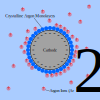
\includegraphics[width=0.5\textwidth]{images/Detector/MalterEffect.pdf}     
    \caption[Malter Effect in Liquid Argon]{A schematic view of the monolayers of crystalline argon a cathode spherical cathode. Attracted by \gls{VanDerWaalsForce}, \ce{Ar} atoms (blue) form an atomic monolayer around metal surfaces, in this case the cathode surface. The negative charge of the cathode attracts \ch{Ar2^+} ions and the monolayer impedes the recombination of the ions with electrons on the cathode surface. Thus, a steep electric field gradient is induced which in turn may trigger an electrical breakdown of the cathode, similar to the Malter effect \cite{MalterEffect}.}
\label{fig:MalterEffect}
\end{figure}
A later study by \gls{fnal} showed a cathode shape dependence of discharge probabilities \cite{LArBreakdownNewFNAL}. In general discharges are a stochastic process and thus the chain of events leading to them is not repeatable, but there still is a general rule for the circumstances they develop. Aforementioned rule predicts the electric breakdown field between the cathode and the ground $E_\text{max}$ as a function of the stressed cathode area $A$ where the electric field exceeds \SI{90}{\percent} of $E_\text{max}$ \cite{LArBreakdownFormula}:
\begin{equation}\label{eq:LArBreakdownFunction}
    E_{\text{max}} = CA^p.
\end{equation}
The constants $C$ and $p$ are used as fit parameters. A combined fit of \gls{lar} breakdown experiments performed at \gls{lhep} \cite{LArBreakdownNew2,LArBreakdownNew1} and \gls{fnal} \cite{LArBreakdownNewFNAL} resulted in $C = \SI{139(5)}{\kilo\volt\per\centi\metre\tothe{3p}}$ and $p=\num{-0.22(1)}$. Said fit of above function and the $E_\text{max}$ measurements cited before are illustrated in figure \ref{fig:LArBreakdownFunction}. As one can see, the data points are broadly scattered around the fit function. The latter acts as a mean and not a limit, \ie if one wants to operate a \gls{lartpc} without discharges, the corresponding $E_\text{max}$ of the fit must be reduced by at least a factor of two.
\begin{figure}[htbp]
    \centering
    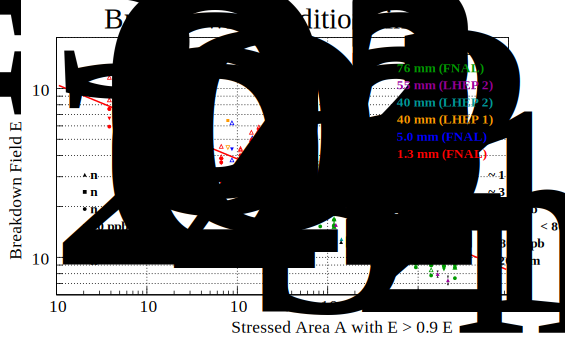
\includegraphics[width=0.9\textwidth]{images/Detector/LArBreakdownFunction.pdf}     
    \caption[Breakdown Field in Liquid Argon as a Function of Stressed Cathode Area]{Breakdown field $E_\text{max}$ as a function of stressed cathode area $A$ with $E > 0.9 E_\text{max}$. The shape of the data points corresponds to different oxygen equivalent impurity levels $n_{O_{2}}$, while the different colours stand for cathode radii used in various experiments. All data points are sourced from three publications: (FNAL) \cite{LArBreakdownNewFNAL}, (LHEP 1) \cite{LArBreakdownNew1} and (LHEP 2) \cite{LArBreakdownNew2}. The red line represents the best fit for equation \ref{eq:LArBreakdownFunction} with parameters $C = \SI{139(5)}{\kilo\volt\per\centi\metre\tothe{3p}}$ and $p = \num{-0.22(1)}$. This illustration is an adapted version sourced from \cite{LArBreakdownNew2}.}
\label{fig:LArBreakdownFunction}
\end{figure}

After the first measurement at \gls{lhep}, we still had questions on how breakdowns actually form. In a second measurement campaign we therefore employed a highspeed camera and an optical spectrometer to analyse the process of the discharge itself \cite{LArBreakdownNew2}. In this study we could identify the three stages of an electrical breakdown in \gls{lar}. The first phase starts with the field emission of electrons from a point on the cathode. Said electrons drift towards the ground, ionising and exciting argon atoms on their way. This process features a visible cone developing between the starting point on the cathode and the ground plate. The cone emits a broad spectrum of light centred around \SI{580}{\nano\metre} (yellow colour). While developing the brightness of the cone increases exponentially, a signature of an avalanche ionisation. Now the produced argon ions drift towards and converge onto the field emission point on the cathode, heating the area significantly above the \gls{bp}. About \SI{2}{\milli\second} after the beginning of the first phase, this occurrence leads to the creation of an argon gas bubble on the cathode surface and thus to the initiation of the second phase. Since argon gas is a better conductor and features a higher avalanche multiplication factor than \gls{lar}, a plasma forms in the bubble. The plasma formation now shields the field emission at the cathode and the cone is quenched. Accelerated electrons in the plasma hit the gas-liquid interface of the bubble causing it to grow and elongate. This formation is called a streamer. Its tip advances on a rambling path in the general direction of the field lines at a velocity of $\sim \SI{300}{\milli\metre\per\second}$. This leads to the growth of a thin and ever longer filament. The streamer has a sharp peak at \SI{700}{\nano\metre} (red) in its emission spectrum, while the advancing tip emits white light (broad spectrum). When the streamer hits the ground plate it establishes a highly conductive channel between cathode and ground. This initiates phase three: the electrical breakdown of the cathode through a spark discharge. The third phase is characterised by a short bright flash, an acoustic shock, and subsequently by intensive bubble formation. The emission spectrum of the breakdown is continuous and dominated by blue and green emissions. The above process can be observed in two videos of breakdowns in \gls{lar} taken at a shutter speed of \SI{1250}{\fps} which are published as data supplements\footnote{\url{http://stacks.iop.org/jinst/11/P03017/mmedia}} of our paper \cite{LArBreakdownNew2}.

For large scale \glspl{lartpc}, with drift lengths of the order of \SI{10}{\metre}, the above discussed breakdown mechanisms poses a major challenge since they will feature cathode voltages of the order of \SI{1}{\mega\volt}. This means that they will feature cathode to ground gaps of the order of \SI{1}{\metre}, leading to a huge unused volumes of \gls{lar}. However, there is a way to increase the breakdown field by coating the cathode in a thin layer of polyisoprene (latex rubber), as discussed in a third \gls{hv} paper from our group \cite{LArBreakdownSuppression}. We measured an electric breakdown filed strength $E_\text{max} = \SI{412}{\kilo\volt\per\centi\metre}$ after applying a layer of \SI{450}{\micro\metre} of polyisoprene. This corresponds to more than a tenfold increase of $E_\text{max}$ compared to a bare metal cathode. This is attributed to the low electron mobility of polyisoprene in the range between \SIrange{e-11}{e-4}{\centi\metre\squared\per\volt\per\second}. This causes the electrons to slowly drift through the material, thus inhibiting the avalanche formation. At the polyisoprene-\gls{lar} interface they recombine with the \ch{Ar2^+} ions, since the crystalline monolayer is only formed on metal surfaces and is thus not present in this setup. This could be the solution for the \gls{hv} problem of \glspl{lartpc}, although after a single breakdown such a coating looses its discharge quenching property.

It took decades until the breakdown issue was acknowledged which I personally attribute to a general shyness and maybe a grain of false pride in our community. It was seen as a failure, if the own experiment could not reach the specified voltages. Therefore, these ``failures'' were not mentioned in publications. Only when meeting people in person at conferences, one was able to share the issues experienced. Still I think the \gls{hv} breakdown investigations were finally a good example of how the \gls{lartpc} community should investigate problems in the field. People from various experiments met at a \gls{hv}-workshop at \gls{fnal}, shared results and their experiences. In my view, this workshop marked a turning point in the \gls{hv} matter and sparked various measurements and investigations.

\section{Cosmic Background Pileup} \label{sec:CosmicPileup}
As mentioned before, the drift of \gls{quasifreeelectron} is a rather slow process and dominates the time span of a \gls{lartpc}'s readout cycle with a duration of the order of \SI{1}{\milli\second}. Competing detector technologies used in neutrino physics experiments, in contrast, exhibit much shorter cycles, around \SI{10}{\nano\second}. This circumstance leads to a particular issue prevalent in \glspl{lartpc}: the cosmic background pileup. Said pileup is the result of cosmic-ray particle interactions in the active volume immediately before a beam related event or during the readout process. Now, let us discuss the mechanisms of said background in an example. First, a cosmic-ray particle enters the \gls{tpc} through the cathode, producing a scintillation \gls{Flash} at a time $t=t_\text{c}$, as shown in figure \ref{fig:CosmicPileup1}. Immediately thereafter, the ionisation track starts to drift towards the anode. If there is a beam related event interacting at the time $t=t_0$ while aforementioned track is still drifting, the now drifted-in track features a loose end within the active volume resembling a \gls{Vertex}, see figure \ref{fig:CosmicPileup2}. Said perceived \gls{Vertex} will be located at a distance $x = v_\text{d}(t_0-t_\text{c})$ from the cathode in the reconstructed event in figure \ref{fig:CosmicPileup4}. If another cosmic-ray particle crosses the chamber through the anode at a time, $t=t_\text{a}$, after the beam related interaction, see figure \ref{fig:CosmicPileup3}, its ionisation track will also be shifted into the active volume during reconstruction. This creates another seeming \gls{Vertex} as shown in figure \ref{fig:CosmicPileup4}.
\begin{figure}[htbp]
    \centering
    \subfloat[Cosmic-Ray Particle Interaction $t_\text{c}$][Cosmic-ray particle interaction at $t_\text{c}$]
    {
        \includegraphics[width=0.48\textwidth]{images/Detector/CosmicPileup1.pdf}
        \label{fig:CosmicPileup1}
    }
    \subfloat[Drifted-in Cosmic Track][Drifted-in track at $t_0$ of a beam related event]
    {
        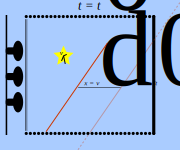
\includegraphics[width=0.48\textwidth]{images/Detector/CosmicPileup2.pdf}
        \label{fig:CosmicPileup2}
    } \\
    \subfloat[Cosmic-Ray Particle Interaction][Another cosmic-ray particle interaction at $t_\text{a}$]
    {
        \includegraphics[width=0.48\textwidth]{images/Detector/CosmicPileup3.pdf}
        \label{fig:CosmicPileup3}
    }
    \subfloat[Reconstructed Beam Event for $t_{0}$][Reconstructed beam event for $t_{0}$]
    {
        \includegraphics[width=0.48\textwidth]{images/Detector/CosmicPileup4.pdf}
        \label{fig:CosmicPileup4}
    }
    \caption[Cosmic Background Pileup]{Above series of figures shows the cosmic background pileup process. \subref{fig:CosmicPileup1} In the beginning at $t=t_\text{c}$, a cosmic particle crosses the active volume of the \gls{tpc} permeating through the cathode. \subref{fig:CosmicPileup2} Then, the ionisation track drifts towards the anode, when suddenly a beam related neutrino interaction occurs at $t=t_0$. \subref{fig:CosmicPileup3} Thereafter, both event signatures drift on as another cosmic-ray particle crosses the chamber, but this time permeating through the anode. \subref{fig:CosmicPileup4} When the event is reconstructed to match the beam event at $t=t_0$, both cosmic-ray related events are mis-projected on the drift axis, seemingly creating fake \glspl{Vertex}. In all four figures, the opaque lines show the position of the charge track at time $t$ and the faint, transparent lines show the true position of the track's origin. The yellow star symbolises the light \gls{Flash} produced by the interactions.}
    \label{fig:CosmicPileup}
\end{figure}
In the domain of \glspl{lartpc}, an event is always reconstructed to the time $t_0$ of a respective beam interaction, wherefore cosmic-ray related background events are usually mis-projected on the drift axis. The pileup of apparent \glspl{Vertex} of cosmic events piercing through anode or cathode constitute one of the major backgrounds of surface detectors with high cosmic-ray flux, like MicroBooNE. Deep underground experiments are naturally not subject to this particular background, as the cosmic-ray flux at their location is heavily reduced. At the time of MicroBooNE's conception, said background was not identified as a problem, although a cosmic-ray muon rate of \SI{5.5}{\kilo\hertz} in the \gls{tpc} leads to an expected \num{13} potential background events in a single readout window of \SI{2.25}{\milli\second} \cite{MicroBooNEMuonRate}. Even more disconcerting, the MicroBooNE proposals \cite{MicroBooNEProposal1, MicroBooNEProposal2} only identified advantages of the \gls{lartpc} technology vis-a-vis a Cherenkov detector, \eg the aforementioned electron-photon discrimination (see section \ref{sec:EnergyDissipationNeutral}). The importance of reducing the cosmic pileup background will be discussed in a small cosmic-ray photon study I performed in chapter \ref{sec:CosmicRayGammaBackground}.

There are, however, two methods to mitigate the above described background. One of these is utilising the light readout system to identify the various scintillation \glspl{Flash} and their origin. Once the \gls{Flash} is matched to its respective charge signal, the latter can be projected correctly to its location of incidence. This so-called \gls{Flash}-matching becomes really challenging with increasing background event numbers, as the misidentification probability of fake \glspl{Vertex} rises \cite{MicroBooNEFlashMatching}. Moreover, there are \glspl{Flash} that are not related to any charge signal, since light readout systems are usually sensitive to more than just the active volume. Depending on the accuracy and method of \gls{Flash}-matching, this background rejection method may lead to a noticeable loss in detector sensitivity, \ie many beam related events get discarded as well. A second method employs tracking detectors outside of the \gls{tpc}. Said external detector needs to be able to tag a cosmic event in space and time in order to correlate it with the \gls{tpc} signals. Such a \gls{crt} system was proposed and built by our group at \gls{lhep} \cite{CRTGeneral}. Cosmic-ray tagging and \gls{Flash}-matching are then combined, in order to increase the matching probability and decrease the beam event rejection. MicroBooNE's \gls{crt} system will be described in detail, later on in this thesis in section \ref{sec:CRT}.

\section{Space Charge Effect} \label{sec:SpaceCharge}
In section \ref{sec:ChargeDrift}, I introduced the rather low \ch{Ar2^+} mobility, $\mu_{0,\text{i}} = \SI{1.5e-3}{\centi\metre\squared\per\volt\per\second}$ which, consequently, leads to long dwell times of said ions in a \gls{tpc}. For a full drift in a \gls{tpc} with several metre drift distance, said dwell times are of the order of \SI{10}{\minute}. Hence, cosmic rays, constantly producing electron-ion pairs in the active volume, lead to an accumulation of continuous clouds of positively charged argon dimers. Such ion clouds are called \textbf{space charge} and were first discovered in the early 1900s in gas diodes \cite{SpaceChargeDiscovery1,SpaceChargeDiscovery2}. If the production of space charge is high enough, it will ultimately lead to distortions in the drift electric field, $\vec{E}$. In noble liquid detectors, said distortions were first observed in liquid krypton calorimeter prototypes for the NA48 experiment at CERN \cite{SpaceChargeDiscovery3}. In the context of these NA48 related measurements, S. Palestini \etal produced a model describing the influence of space charge on the drift field \cite{LArSpaceCharge1}, which I will later discuss here in more detail. In \gls{lar}, the space charge effect was first observed in a thin-gap ionisation chamber \cite{LArSpaceChargeDiscovery}. Both these noble liquid experiments featured short drift distances of \SI{1}{\centi\metre} and \SI{100}{\micro\metre}, respectively. Hence, the respective detectors had to be subject to intense radiation, in order for the space charge effect to become noticeable. For \glspl{lartpc} with drift distances of several metres, the effect becomes perceivable at much lower activity. For surface detectors with small overburden, even cosmic radiation is enough to induce the effect, as MicroBooNE has shown \cite{LArLaserMicroBooNE1,LArLaserMicroBooNE2,LArSpaceChargeMicroBooNE}. The MicroBooNE collaboration came up with their own, simplified model to describe the influence of space charge on the drift field. Unfortunately, the collaboration failed to explain the thinking behind said model and contrast it to the work of Palestini \etal. I would like to resolve this deficiency in this section.

First let us quantify said space charge effect on the electric field with the Palestini model. Palestini \etal \cite{LArSpaceCharge1,LArSpaceCharge2} realised that the space charge density has to follow the continuity equation,
\begin{equation}
    \frac{\partial \rho_\text{i}}{\partial t} + \vec{\nabla}\cdot \vec{j}_\text{i} = J.
\end{equation}
Here, $\rho_\text{i}$ stands for the ion density, $\vec{j}_\text{i}$ for the ion flux, and $J$ for the source, \ie the ion generation per unit volume per unit time. In our case, $J$ is deemed to be constant in time and position, as it is determined by the constant flux of cosmic-rays traversing the active volume. The term $\partial \rho_\text{i}/\partial t$ represents the time dependent variation of the charge density and finally $\vec{\nabla}\cdot \vec{j}_\text{i}$ describes the flow of ions, \ie how the charge carriers are transported out of the active volume by their drift. Since the space charge is considered in a velocity field, we can define the flux as $\vec{j}_\text{i} = \rho_\text{i}\vec{v}_\text{i}$. Furthermore, we can simplify above equation, if we think of the \gls{tpc} as an infinite parallel plate capacitor. In that case, $\rho_\text{i}$ and $\vec{v}_\text{i}$ only exhibit a drift coordinate, $x$, dependency. Hence, we reduce the problem to one dimension and replace $\vec{v}_\text{i}$ with $v_x$. Moreover, due to the constant generation of ions, $J$, the space charge concentration in the detector is expected to become stable after a certain time of operation. This stationary solution of the continuity equation, \ie $\partial \rho_\text{i} / \partial t = 0$, is of particular interest, for it describes the equilibrium state all \glspl{tpc} are operated in. Thus, above equation takes the form
\begin{equation} \label{eq:ContinuityEquation}
    \frac{\partial(\rho_\text{i} v_x)}{\partial x} = J.
\end{equation} 
Now we can use the mobility relation for the drift velocity, $v_x = \mu_{0,\text{i}} E_x$ from equation \ref{eq:DriftVelocity}, and integrate
\begin{align} \label{eq:StationaryContinuityEq}
    \int d(\rho_\text{i} E_x)\ \mu_{0,\text{i}} &= \int dx\ J, \nonumber \\[5pt]
    \Longrightarrow \ \mu_{0,\text{i}} \rho_\text{i} E_x &= J x + A.
\end{align}
Here $E_x$ stands for the drift coordinate component of the electric field, and $A$ for the integration constant. At the anode, \ie $x=0$, we expect $\rho_\text{i} = 0$, and thus get $A = 0$ as well. In order to obtain the connection between $\rho_\text{i}$ and $E_x$, it is useful to employ the \gls{1d} form of the first Maxwell equation, 
\begin{equation} \label{eq:MaxwellEquation1D}
    \frac{\partial E_x}{\partial x} = \frac{\rho_\text{i}}{\epsilon_0\epsilon_\text{r}},
\end{equation}
with $\epsilon_0\epsilon_\text{r}$ again representing the dielectric constant of \gls{lar}. By replacing $\rho_\text{i}$ of equation \ref{eq:StationaryContinuityEq}, we arrive at our final, solvable differential equation for $E_x$ with
\begin{equation}
    \epsilon_0\epsilon_\text{r}\mu_{0,\text{i}}E_x\frac{\partial E_x}{\partial x} = J x.
\end{equation}
Solving above equation with the proper boundary conditions for the integration constants results in \cite{LArSpaceCharge1}
\begin{equation} \label{eq:PalestiniField}
    E_x(x) = E_0 \sqrt{\left(\frac{E_\text{a}}{E_0}\right)^2 + \alpha^2 \left(\frac{x}{L}\right)^2}, \qquad \text{with} \quad \alpha = \frac{L}{E_0}\sqrt{\frac{J}{\epsilon_0\epsilon_\text{r}\mu_{0,\text{i}}}}.
\end{equation}
In above equation, $E_0$ denotes the electric field strength without space charge, $E_\text{a}$ the field strength at the anode (with space charge), and $L$ the full drift distance of the \gls{tpc}. The electric field at the anode, $E_\text{a}$, can be calculated using the boundary condition given by the applied cathode voltage $V_0$
\begin{equation} \label{eq:AnodeBoundaryCondition}
    V_0 = -\int_{0}^{L} dx \ E_x(x).
\end{equation}
Since above integral leaves us with no analytical solution for $E_\text{a}$, there is an numerical approximation given by \cite{LArSpaceCharge2}
\begin{equation}
    E_\text{a} = 
    \begin{cases}
        E_0\left( 1-\alpha^2/6-\alpha^4/180 \right) & \text{for} \ \alpha < 1.57 \\
        E_0\left( 1-\alpha^2/6-\alpha^4/180-\alpha^6/8500 \right) & \text{for} \ \alpha < 1.89
    \end{cases},
\end{equation}
For $\alpha > 2$, the Palestini model reaches its limit as $E_\text{a} < 0$, \ie the charge density gets high enough, that the electric field at the anode would reverse. In case of such an extreme space charge concentration in the active volume, the \gls{tpc} would simply cease functioning. With $E_x(x)$ established, it is then quite simple to derive the charge density distribution, $\rho_\text{i}(x)$ by again making use of the \gls{1d} Maxwell equation \ref{eq:MaxwellEquation1D} and get
\begin{align}
    \rho_\text{i}(x) &= \epsilon_0\epsilon_\text{r}\,\frac{\partial E_x(x)}{\partial x} \nonumber \\
    &= \alpha^2 \epsilon_0\epsilon_\text{r} \, \frac{E_0^2}{E_x(x)} \frac{x}{L^2}.
\end{align}

MicroBooNE's approach assumes the space charge density to be linear in the drift coordinate, $x$, \ie $\rho_\text{i}(x) = a x$ \cite{LArSpaceChargeMicroBooNE}. Even before MicroBooNE, I myself used the same linear approximation in my master's thesis \cite{LArTPCMasterChristoph}. It is the logical first order solution, if one considers a constant drift velocity and a constant ionisation rate in the chamber. However, myself and the MicroBooNE collaboration failed to connect this assumption to the continuity equation, as we did not research the topic properly. The key difference between the MicroBooNE approximation and the Palestini model is the assumption that $v_x$ is constant. All other assumptions stay the same. Pertaining the continuity equation in \ref{eq:ContinuityEquation}, MicroBooNE's first order approximation takes the form
\begin{align}
    v_x\,\frac{\partial\rho_\text{i}}{\partial x} &= J, \nonumber \\
    \Longrightarrow \ \rho_\text{i}(x) &= \frac{J}{v_x}x
\end{align}
The integration constant of above relation equates to zero, as $\rho_\text{i}(0) = 0$. From here MicroBooNE uses \gls{3d} numerical integration in order to get to the solution for the electric field. Since I would like to compare the MicroBooNE approximation to the Palestini model, I proceed to calculate $E_x$ using equation \ref{eq:MaxwellEquation1D} and get
\begin{align}
    E_x(x) &= \int dx \ \frac{\rho_\text{i}(x)}{\epsilon_0\epsilon_\text{r}} \nonumber \\
           &= E_\text{a} + \frac{J}{2v_x\epsilon_0\epsilon_\text{r}}x^2.
\end{align}
Here I also used the boundary condition at $x=0$ to determine the integration constant as $E_\text{a}$. This time, however, $E_\text{a}$ can be obtained analytically by solving equation \ref{eq:AnodeBoundaryCondition} like
\begin{align}
    V_0 &= -\int_{0}^{L} dx \ E_x(x), \nonumber \\
        &= -E_\text{a} L - \frac{J}{6v_x\epsilon_0\epsilon_\text{r}} L^3, \nonumber \\[5pt]
    \Longrightarrow \ E_\text{a} &= E_0 - \frac{J}{6v_x\epsilon_0\epsilon_\text{r}} L^2.
\end{align}
In the last step of above derivation, I used the relation $E_0 = -V_0/L$. With both models established, we can now compare their solutions for $\rho_\text{i}(x)$ and $E_x(x)$, shown in figure \ref{fig:SpaceChargeModels}, using MicroBooNE's detector specifications. MicroBooNE exhibits a space charge source of $J = \SI{1.6e-10}{\coulomb\per\metre\cubed\per\second}$ \cite{LArSpaceChargeMicroBooNE}, a cathode voltage of $V_0 = \SI{-70}{\kilo\volt}$, a full drift length of $L = \SI{256}{\centi\metre}$, and thus an electric field strength without space charge of $E_0 = \SI{273.4}{\volt\per\centi\metre}$.
\begin{figure}[htbp]
    \centering
    \subfloat[Space Charge Density][Space charge density]
    {
        \includegraphics[width=1.0\textwidth]{images/Detector/SpaceChargeDensity.pdf}
        \label{fig:SpaceChargeDensity}
    } \\
    \subfloat[Electric Field Distortion due to Space Charge][Electric field distortion due to space charge]
    {
        \includegraphics[width=1.0\textwidth]{images/Detector/SpaceChargeField.pdf}
        \label{fig:SpaceChargeField}
    }
    \caption[Space Charge Models]{These graphs illustrate the Palestini model and the MicroBooNE approximation of the space charge density $\rho_\text{i}(x)$ \subref{fig:SpaceChargeDensity} and the resulting electric field strength on the drift axis $E_x(x)$ \subref{fig:SpaceChargeField}. In order to emphasise the field distortions introduced by space charge, the constant design field strength $E_0$ is shown as a red line in \subref{fig:SpaceChargeField}. All models are drawn, using MicroBooNE detector specifications.}
    \label{fig:SpaceChargeModels}
\end{figure}
% TODO add correlation factor?
As can be seen in figure \ref{fig:SpaceChargeDensity}, MicroBooNE's approximation of the Palestini model and the Palestini model itself are quite close for $x<\SI{150}{\centi\metre}$, concerning the space charge density. Thereafter, towards the cathode, they start to diverge with a maximum $\rho_\text{i}(x)$ difference of $\sim\SI{20}{\percent}$. However, this difference is much smaller when considering $E_x(x)$ of both models, as shown in figure \ref{fig:SpaceChargeField}. As an approximation for $E_x(x)$, MicroBooNE's approach is certainly usable, although the Palestini model is still preferable in my opinion, since it is more accurate and does not complicate calculations significantly, \ie why simplify a model that is already simple to solve. Comparing the two field strength curves $E_x(x)$ to the constant $E_0$ in \ref{fig:SpaceChargeField}, it becomes obvious how space charge distorts the field. It lowers $E_x(x)$ at the anode, but leads to an increase at the cathode. As stated before, both models do not take into account the field components in the $y$ and $z$ coordinates. Therefore, both models are only valid in the very centre of the detector's $y$-$z$ coordinates, for the field cage elements introduce non-zero values for $E_y$ and $E_z$. Thus, the MicroBooNE collaboration's decision to use full \gls{3d} integration of the charge density in order to determine the electric field is certainly increasing the accuracy of the model. Furthermore, non-zero values for $E_y$ and $E_z$ also means non-zero values for $v_y$ and $v_z$ which in turn again influences the charge density distribution. Still, if $E_{y,z} \ll E_x$, the effect on the space charge density might be minimal. One open point that remains unaddressed, is the change in the flux $\vec{j}$, or $\vec{v_i}$ respectively, due to fluid currents in \gls{lar}. Said currents are induced by convection and the recirculation of \gls{lar} and are of the same order of magnitude as the drift velocity. These partially random currents are very difficult to measure or simulate. Hence, there might never be a complete model to describe the space charge effect in a \gls{lartpc}.

It is impossible to compensate for the space charge effect in a \gls{tpc} with adaptations of the field cage design, because of the randomness of the \gls{lar} flow. The only way to mitigate the severity of the effect is to choose a small drift distance. Since this would also increase the numbers of readout channels for the instrumentation of the same volume, smaller drifts are often not preferable. However, the drift field distortion, caused by space charge, can be measured using the ionisation track of an \gls{uv} laser beam as introduced in section \ref{sec:MultiPhotonIonisation}. The positional distortion of the recorded events can be directly measured as the displacement of the laser track within the active volume. For this to work, the true position and direction of the laser beam needs to be determined to high accuracy. Said true track then has to be compared, in a discrete manner, with the apparent position of the reconstructed track after completion of the \gls{tpc}'s readout process. In such an arrangement, the \gls{3d} displacement vector is then defined as
\begin{equation} \label{eq:DisplacementDefinition}
    \vec{d}_i \coloneqq \vec{t}_i - \vec{r}_i,
\end{equation}
where $i$ denotes the index of a discrete reconstructed track point, $\vec{r}_i$, and its associated position on the true laser track, $\vec{t}_i$. There is, however, a problem: we only know two parameters of the true laser track, the entry point, $\vec{L}_\text{entry}$, and the exit point, $\vec{L}_\text{exit}$, from the active volume. This leads to ambiguities for the true position, $\vec{t}_i$, as in principle every position along the true track between $\vec{L}_\text{entry}$ and $\vec{L}_\text{exit}$ could be chosen. Yet, $\vec{t}_i$ can be approximated, assuming the displacement, $\vec{d}_i$, to be minimal, \ie $\vec{d}_i \perp (\vec{L}_\text{exit} - \vec{L}_\text{entry})$. Therefore, we can rewrite equation \ref{eq:DisplacementDefinition} as
\begin{equation} \label{eq:DisplacementEquation}
    \vec{d}_i = \vec{L}_\text{entry} + \alpha_i\left(\vec{L}_\text{exit} - \vec{L}_\text{entry}\right) - \vec{r}_i.
\end{equation}
Since, in our example, the displacement is perpendicular to the true laser track, we can use $\vec{d}_i \cdot (\vec{L}_\text{exit} - \vec{L}_\text{entry}) = 0$ to solve for the scaling factor $\alpha_i$, resulting in
\begin{equation}
    \alpha_i = \frac{\left(\vec{r}_i - \vec{L}_\text{entry}\right) \cdot \left(\vec{L}_\text{exit} - \vec{L}_\text{entry}\right)}{\left\vert\vec{L}_\text{exit} - \vec{L}_\text{entry}\right\vert^2}.
\end{equation}
Other approximation methods, \eg $\vec{d}_i \perp \vec{r}_i$, would lead to other constraints and hence different solutions for $\alpha_i$. A \gls{2d} representation of the above-described procedure to determine the displacement is shown in figure \ref{fig:LaserCallibrationMethod}.
\begin{figure}[htbp]
    \centering
    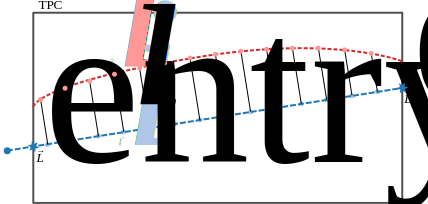
\includegraphics[width=\textwidth]{images/Detector/LaserCallibrationMethod.pdf}
    \caption[Displacement Measurement Method]{Shown here, is a schematic view of a displacement measurement method employing a laser system in \gls{lar}. The true laser path is shown in blue, and the due to space charge distorted \gls{quasifreeelectron} track in red. Above figure was originally drawn by M. L\"uthi for his PhD Thesis \cite{LArLaserPhDMatthias} and slightly adapted.}
    \label{fig:LaserCallibrationMethod}
\end{figure}
Whichever method is chosen, the ambiguities on the beam axis can not be avoided, but there are no ambiguities in the plane perpendicular to the true track. Thus, a second laser beam, ideally perpendicular to the first one, can mitigate or even resolve these ambiguities. Said mitigation is done iteratively by correcting the track of the first laser in small steps with the displacement measured by the second one, and vice versa. Moreover, movable mirrors, as used in MicroBooNE, are able to provide a multitude of laser tracks with different angles which therefore cover a large part of the active volume.

With these vast amounts of recorded laser tracks, one receives a large set of irregularly spaced reconstructed points, $\vec{r}_{n,m}$, each with a displacement vector, $\vec{d}_{n,m}$. Here, $n$ is the track number and $m$ the track point index introduced above. This irregularity is unfavourable for our purpose, as we aim to not only reconstruct the displacement, but also the electric field. Hence, an equally spaced \gls{3d} grid, called displacement map, needs to be created by applying an elaborate interpolation algorithm. Said algorithm first creates a mesh of all irregular points employing Delaunay refinement. Then, the regular grid points are interpolated using barycentric coordinates within the mesh. I will skip the exact formalism of this procedure in this work, for it is already documented in great detail \cite{LArLaserMicroBooNE2,LArLaserPhDMatthias,LArLaserPhDYifan}.

In this regular grid, called displacement map, we now end up with three indices for all three dimensions, $i$ for the $x$, $j$ for the $y$, and $k$ for the $z$-component of the map. The displacement vector is therefore denoted as $\vec{d}_{i,j,k}$. The spacing of the grid points is, as mentioned before, regular with a size of $\Delta x$. On the drift axis ($x$-axis) the grid spacing is connected to the drift time,$\Delta t$ by $\Delta x = v_\text{d}\Delta t$, with $v_\text{d}$ denoting the constant drift velocity of the \gls{quasifreeelectron} disregarding field distortions. Now, in order to reconstruct the drift electric field, we first need to derive the drift velocity from the displacement map. This is done in reverse to the drift process, starting at the anode and ending at the cathode, using the displacement difference of two adjacent points on the drift axis
\begin{equation} \label{eq:DisplacementDifference}
    \vec{R}_{i,j,k} \coloneqq \vec{d}_{i+1,j,k} - \vec{d}_{i,j,k}.
\end{equation}
As a matter of fact, $\vec{R}_{i,j,k}$ describes the movement of the drifted charge carriers within the time window $\Delta t$. From this it is straight forward to evaluate the drift velocity for each grid point as
\begin{align} \label{eq:VelocityDistortion}
    \vec{v}_{i,j,k} &= -\frac{1}{\Delta t} \vec{R}_{i,j,k}, \nonumber \\[5pt]
    \Longrightarrow \ \vec{v}_{i,j,k} &= -\frac{v_\text{d}}{\Delta x} \vec{R}_{i,j,k}.
\end{align}
As can be seen, the drift velocity points in the opposite direction of the displacement difference. Furthermore, above method assumes a constant displacement and hence a constant drift velocity within two grid points. Said assumption is valid, if $\Delta x$ is smaller than the expected magnitude of $\vec{d}$. The above described calculation are visualised as a simplified \gls{2d} depiction in figure \ref{fig:LaserVelocityCallibration}.
\begin{figure}[htbp]
    \centering
    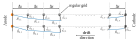
\includegraphics[width=\textwidth]{images/Detector/LaserVelocityCallibration.pdf}
    \caption[Drift Velocity Distortion Measurement Method]{Depicted here is the drift velocity distortion measuring method as a \gls{2d} simplification. It uses the displacement differences $\vec{R}_{i,j}$ in a regular grid and applies them to equation \ref{eq:VelocityDistortion}. Again, the original is sourced from M. L\"uthi's Thesis \cite{LArLaserPhDMatthias} and slightly altered.}
    \label{fig:LaserVelocityCallibration}
\end{figure}
From here, it is quite simple to calculate the electric field map, $\vec{E}_{i,j,k}$ by using $\vec{v}_{i,j,k}$ and solving the mobility relation of equation \ref{eq:DriftVelocity}. For small field deviations we can even use a constant mobility, in order to simplify calculations. With the displacement, and field maps established, we can now correct particle track positions as well as drift field related effects like recombination. In a surface detector exhibiting the dimensions of MicroBooNE, displacements reach about \SI{15}{\centi\metre} and electric field distortions are found in the vicinity \SI{30}{\volt\per\centi\metre} \cite{LArLaserMicroBooNE2}.

During my time with MicroBooNE, the electric field and displacement calibration became my main task, especially the analysis side. I wrote the software which calculates the displacement and interpolates the grid points. Still, I decided to only include this small summary of this topic, as my colleagues brought the analysis methods to their final form and documented them well in their excellent theses \cite{LArLaserPhDMatthias,LArLaserPhDYifan}.
\end{fmffile} % Close the feynman diagram file
